\documentclass[a4paper]{article}
\usepackage[pdftex]{graphicx}
\usepackage{amsmath,amssymb}
\usepackage{gensymb}
\usepackage{natbib,aas_macros}
\usepackage [english]{babel}
\usepackage{tabu}
\usepackage[toc,page]{appendix}
\usepackage{subcaption}

%choose margin size
\usepackage[margin=1in]{geometry}
\usepackage{float}
\usepackage{hyperref}

%allow roman numerals
\newcommand{\RN}[1]{%
  \textup{\uppercase\expandafter{\romannumeral#1}}%
}

\usepackage{hyperref}
\setcounter{tocdepth}{1} % set table of contents to only include part,chapters,sections (from https://tex.stackexchange.com/questions/291307/how-to-hide-show-section-levels-in-the-table-of-contents)

\newcommand{\ph}{\phantom}
\newcommand{\alp}{\alpha}
\newcommand{\Gam}{\Gamma}
\newcommand{\gam}{\gamma}
\newcommand{\pd}{\partial}
\newcommand{\mesc}{\texttt{mescaline}}
\newcommand{\avgb}[1]{\langle #1 \rangle^b_D}
\newcommand{\avg}[1]{\langle #1 \rangle_D}
\newcommand{\mfkh}{\mathfrak{h}}
\newcommand{\dtwoh}{\frac{{\rm d}^2\mfkh}{{\rm d}s^2}}




%fix quotation marks
\usepackage [autostyle, english = american]{csquotes}
\MakeOuterQuote{"}

\newcommand{\HRule}{\rule{\linewidth}{0.5mm}}
\savegeometry{origin}
\geometry{rmargin=1in,lmargin=1in}


\title{\texttt{Mescaline}: User(s) guide}
\author{Hayley J. Macpherson}

\begin{document}
\maketitle

\texttt{Mescaline} is an analysis code written in Fortran by Daniel Price and Hayley Macpherson for post-processing analysis of Cactus data -- specifically intended for inhomogeneous cosmology. It calculates various tensors, vectors, and scalars for interpreting the general-relativistic effects on an inhomogeneous, anisotropic spacetime. See \citet{macpherson2018b,macpherson2019b} for some applications of the code. 

In this document we outline the basics of getting set up with certain dependencies, compiling, and using \mesc. We also give details on what is actually calculated, including equations, methods, explanations, etc., of the way certain things are implemented. We also include some consistency tests at the end using analytic metrics.



\tableofcontents


%----------------------------------------------------------------------------------
\section{Usage}
%----------------------------------------------------------------------------------

\mesc\, reads in HDF5 file format as (almost) written by the Einstein Toolkit (ET). 

The ET writes data in variable-chunked format, i.e., one file per variable containing every time step. Because of this format, these files can get very large and difficult to deal with for bigger simulations.
In \mesc\texttt{/tools/} directory we include a Python script \texttt{split\_HDF5\_per\_iteration3.py} to split these files into a more manageable format. This splits the ET output HDF5 data (e.g., \texttt{rho.xyz.h5}) into iteration-chunked data, i.e. a single file for each time step containing all variables in the simulation directory. The format resulting from this script is the format that \mesc\ can read.

First, run this script from your simulation directory. Note this might take a while for larger simulations, however, it only needs to be done once. 

See the README for simple instructions to get started. We elaborate on some of these details here.
%----------------------------------
\subsection{Dependencies}
%----------------------------------

\subsubsection{SPLASH}

SPLASH is a visualisation tool for SPH simulations, written by Daniel Price. You first must download the most recent version of SPLASH, since \mesc\, borrows some of its modules for reading HDF5 data. See \href{http://users.monash.edu.au/~dprice/splash/}{here} for download and installation instructions, or, just use Homebrew:

\vspace{2mm}
\texttt{brew tap danieljprice/all} \\

\texttt{brew install splash}
\vspace{2mm}

Once that is done, make sure you have set the environment variable \texttt{SPLASH\_DIR} to the location of your \texttt{splash/} directory, e.g. 

\vspace{2mm}
\texttt{export SPLASH\_DIR=~/splash}.
\vspace{2mm}

Note that SPLASH can also be used to visualise ET output data (using the split files) by compiling (after a normal compile) with \texttt{make SYSTEM=gfortran cactus}, which will give you an executable \texttt{csplash-hdf5} which can then be used to read Cactus HDF5 data. Email me for more details on this if you need, since it's not documented on the SPLASH pages (I think). Note that you don't actually need to compile SPLASH to be able to run \mesc, you just need the codes there and \texttt{SPLASH\_DIR} pointing to them. \mesc\ will do the rest.

\subsubsection{HDF5}

You need to have HDF5 installed to read (and write) HDF5 files. You will need to set the environment variable \texttt{HDF5ROOT} to the location of your HDF5 root directory, as this is used during compilation of \mesc. 

\subsubsection{C and Fortran compilers}

\mesc\, has been tested to compile using both GNU and Intel compilers (though different versions may behave differently). Set the environment variable \texttt{SYSTEM}=\texttt{gfortran} or \texttt{SYSTEM}=\texttt{ifort} before compiling to choose GNU or Intel compilers, respectively. 


%----------------------------------
\subsection{Compiling}
%----------------------------------

Make sure you set your desired options in \texttt{src/options.f90} \textit{before} compiling. Make sure to \texttt{make clean} and \texttt{make} again when changing \texttt{any} options in here, otherwise the changes won't be propagated to modules that may not be re-compiled with a simple \texttt{make}.

{\bf To compile, type \texttt{make}. This will generate an executable in \texttt{bin/mescaline}.}



%----------------------------------
\subsection{Running}
%----------------------------------

To run \mesc\, first make sure that the options you have set align with the simulation data you are presenting. If not, you could get weird results. 

You can either give \mesc\, a long list of files, or a single file (again, so long as the options are consistent). You {\bf should} get various errors for most of the inconsistencies I've come across -- if you find one that you think needs a flag, please let me know!

The general usage is simple, e.g.

\vspace{2mm}
\texttt{mescaline *.hdf5}
\vspace{2mm}


%----------------------------------------------------------------------------------
\section{Assumptions}\label{sec:assumptions}
%----------------------------------------------------------------------------------

There are a few simple assumptions in \texttt{mescaline}, as follows:
\begin{enumerate}
	\item geometric units with $G=c=1$
	\item a uniform cubic computational grid with ${\rm dx = dy = dz}$ and hence ${\rm nx = ny = nz}$	
	\item periodic boundary conditions implemented when taking all derivatives
	\item gauge enforced such that the shift vector $\beta^i=0$, with $\pd_t \beta^i = 0$
	\item the evolution of the lapse is left general in all calculations (with choices in \texttt{options.f90}), and a routine specifying the form of $\pd_t \alp$ can be changed to whatever you like in \texttt{get\_dtalp} in \texttt{analytic\_solns.f90}
\end{enumerate}

%----------------------------------------------------------------------------------
%----------------------------------------------------------------------------------
\section{Technical details}
%----------------------------------------------------------------------------------
%----------------------------------------------------------------------------------


%----------------------------------------------------------------------------------
\subsection{Definition and notations}
%----------------------------------------------------------------------------------

We use Greek letters to denote spacetime indices which take values $0\ldots 3$, and Latin indices for spatial indices which take values $1\ldots 3$, and summation over repeated indices is assumed. $\nabla_\alp$ is the covariant derivative associated with the metric $g_{\mu\nu}$, and $D_i$ is the spatial covariant derivative associated with the spatial metric $\gam_{ij}$. See \citet{macpherson2019c} for a breakdown of the $3+1$ foliation of spacetime, as notation should be relatively consistent here. $\pd_\alp \equiv \pd / \pd x^\alp $ is the partial derivative with respect to coordinate $x^\alp=(ct,x^i)$.


%----------------------------------------------------------------------------------
\subsection{Averaging in general foliations}
%----------------------------------------------------------------------------------


\citet{buchert2018b,buchert2019} describe their new mass-preserving, fluid-intrinsic averaging formalism for general spacetime foliations. Here we outline some specifics related to how this is implemented in \texttt{mescaline}.


%---------------------------------------
%\subsubsection{Key calculations}
%---------------------------------------

%Here we outline the specifics of the main calculations of the fluid variables. 
See \citet{macpherson2019c} for some details of calculating the spatial Ricci tensor, scalar, trace of the extrinsic curvature, Christoffel symbols. These might be included here later, but they are just spatial derivatives of the metric, so maybe this is self-explanatory. 

%----------------
\subsubsection{Expansion scalar}
%\vspace{5mm}
%\textit{Expansion scalar}
%\vspace{5mm}
%----------------

The expansion scalar $\Theta$ is defined by
\begin{equation}\label{eq:expansion_scalar_defn}
	\Theta \equiv \nabla_\alp u^\alp,
\end{equation}
where $\nabla_\alp$ is the covariant derivative associated with the metric, and $u^\alp$ is the four-velocity of the fluid. This becomes
\begin{equation}
	\Theta = \pd_\alp u^\alp + {}^{(4)}\Gam^\alp_{\alp\beta} u^\beta,
\end{equation}
where ${}^{(4)}\Gam^\alp_{\alp\beta}$ are the four-dimensional Christoffel symbols. Expanding these sums we find 
\begin{equation}
	\Theta = \pd_0 u^0 + \pd_i u^i + \frac{u^0}{\alp} \pd_0 ( \alp ) - \alp K u^0 +   \frac{1}{\alp} \pd_i ( \alp ) u^i + \Gam^j_{ji} u^i,
\end{equation}
where we can write
\begin{equation}\label{eq:pd0u0}
	\pd_0 u^0 = - \frac{1}{\alp^2} \pd_0 u_0 + \frac{2u_0}{\alp^3} \pd_0 \alp,
\end{equation}
and therefore
\begin{equation}
	\Theta = \pd_i u^i - \frac{1}{\alp^2} \pd_0 u_0 - \frac{u^0 }{\alp} \pd_0 ( \alp )- \alp K u^0 +   \frac{1}{\alp} \pd_i ( \alp ) u^i + \Gam^j_{ji} u^i.
\end{equation}
In the above, we have omitted the ${}^{(4)}$ from the spatial parts of the Christoffel symbols since when $\beta^i=0$ these are equivalent to those associated with the three-metric $\gam_{ij}$. We have also used the time components of the four-dimensional Christoffel symbols, namely
\begin{align}
	{}^{(4)}\Gamma^0_{00} &= \frac{1}{\alp}\pd_0 \alp, \quad {}^{(4)}\Gamma^0_{0i} = \frac{1}{\alp}\pd_i\alp, \quad {}^{(4)}\Gamma^0_{ij} = - \frac{1}{\alp} K_{ij}, \\
	{}^{(4)}\Gamma^i_{00} &= \alp \gam^{ij} \pd_j \alp, \quad {}^{(4)}\Gamma^i_{0k} = -\alp K^i_{\ph{i}k},
\end{align}
in deriving the above (and below).

The expansion scalar is currently calculated in \texttt{get\_expansion\_shear\_vort} in \texttt{roots.f90}.

%----------------
\subsubsection{Shear tensor}
%\vspace{5mm}
%\textit{Shear tensor}
%\vspace{5mm}
%----------------

The shear tensor is defined as
\begin{equation}\label{eq:sigma_defn}
	\sigma_{\mu\nu} \equiv b^\alp_{\ph{\alp}\mu} b^\beta_{\ph{\beta}\nu} \nabla_{(\alp} u_{\beta)} - \frac{1}{3}\Theta b_{\mu\nu},
\end{equation}
where the projection tensor is 
\begin{equation}\label{eq:bproj}
	b_{\mu\nu}=g_{\mu\nu} + u_\mu u_\nu,
\end{equation}
and the round brackets indicate symmetrisation over the contained indices. Expanding the covariant derivative and simplifying gives
\begin{equation}
	\begin{aligned}
		\sigma_{\mu\nu} = b^0_{\ph{0}\mu} &b^0_{\ph{0}\nu}  \left( \pd_0 u_0 - \Gam^\alp_{00} u_\alp \right) + \frac{1}{2} \left( \pd_0 u_i + \pd_i u_0 - 2 \Gam^\alp_{0i} u_\alp \right) \left( b^0_{\ph{0}\mu} b^i_{\ph{0}\nu} + b^i_{\ph{i}\mu} b^0_{\ph{0}\nu} \right) \\
					& + \frac{1}{2} b^i_{\ph{i}\mu} b^j_{\ph{j}\nu} \left( \pd_i u_j + \pd_j u_i - 2 \Gam^\alp_{ij} u_\alp \right) - \frac{1}{3}\Theta b_{\mu\nu}.
	\end{aligned}
\end{equation}
The rate of shear is then $\sigma^2 \equiv 1/2 \sigma_{\mu\nu} \sigma^{\mu\nu}$. We note that since $b_{\mu\nu}$ is not the three metric describing the simulation hypersurfaces then the components $\sigma_{00}, \sigma_{0i} \neq 0$. These components are

\begin{equation}
	\begin{aligned}
		\sigma_{00} = \left(b^0_{\ph{0}0}\right)^2 &\left( \pd_0 u_0 - \Gam^\alp_{00} u_\alp \right) + b^0_{\ph{0}0} b^i_{\ph{i}0} \left( \pd_0 u_i + \pd_i u_0 - 2 \Gam^\alp_{0i} u_\alp \right) \\
		&+ \frac{1}{2} b^i_{\ph{i}0} b^j_{\ph{j}0} \left( \pd_i u_j + \pd_j u_i - 2 \Gam^\alp_{ij} u_\alp \right) - \frac{1}{3}\Theta b_{00},
	\end{aligned}
\end{equation}

where

\begin{equation}
	b^0_{\ph{0}0} = 1 - \Gam^2, \quad b^i_{\ph{i}0} = - \alp \Gam u^i, \quad b_{00} = \alp^2 \left( \Gam^2 - 1 \right),
\end{equation}
and
\begin{equation}
	\begin{aligned}
		\sigma_{0i} = b^0_{\ph{0}0} b^0_{\ph{0}i} &\left( \pd_0 u_0 - \Gam^\alp_{00} u_\alp \right) +  \frac{1}{2} \left( b^0_{\ph{0}0} b^k_{\ph{0}i} + b^k_{\ph{k}0} b^0_{\ph{0}i} \right) \left( \pd_0 u_k + \pd_k u_0 - 2 \Gam^\alp_{0k} u_\alp \right) \\
		&+ \frac{1}{2} b^k_{\ph{k}0} b^j_{\ph{j}i} \left( \pd_k u_j + \pd_j u_k - 2 \Gam^\alp_{kj} u_\alp \right) - \frac{1}{3}\Theta b_{0i},
	\end{aligned}
\end{equation}
where
\begin{equation}
	b^0_{\ph{0}i} = u^0 u_i, \quad b_{0i} = - \alp^2 u^0 u_i.
\end{equation}

The shear tensor (and scalar) is currently calculated in \texttt{get\_expansion\_shear\_vort} in \texttt{roots.f90}.


%----------------
\subsubsection{Vorticity tensor}
%\vspace{5mm}
%\textit{Vorticity tensor}
%\vspace{5mm}
%----------------

The vorticity tensor is defined as
\begin{equation}
	\omega_{\mu\nu} \equiv b^\alpha_{\ph{\alpha}\mu} b^\beta_{\ph{\beta}\nu} \nabla_{[\alpha} u_{\beta]}
\end{equation}
where the square brackets imply anti-symmetrisation across the enclosed indices, i.e.
\begin{equation}
	\omega_{\mu\nu} = b^\alpha_{\ph{\alpha}\mu} b^\beta_{\ph{\beta}\nu} \frac{1}{2} \left( \nabla_\alpha u_\beta - \nabla_\beta u_\alpha \right),
\end{equation}
expanding the covariant derivative we find
\begin{align}
	\omega_{\mu\nu} &= b^\alpha_{\ph{\alpha}\mu} b^\beta_{\ph{\beta}\nu} \frac{1}{2} \left( \pd_\alpha u_\beta - \Gamma^\gamma_{\alpha\beta} u_\gamma - \pd_\beta u_\alpha + \Gamma^\gamma_{\alpha\beta} u_\gamma \right), \\
				&= b^\alpha_{\ph{\alpha}\mu} b^\beta_{\ph{\beta}\nu} \frac{1}{2} \left( \pd_\alpha u_\beta - \pd_\beta u_\alpha \right),
\end{align}
i.e. the symmetric parts (Christoffel symbols) cancel. The vorticity scalar is then $\omega^2 \equiv (1/2)\, \omega_{\mu\nu} \omega^{\mu\nu}$.

The components, as calculated in \mesc, are
\begin{align}
	%\omega_{00} &= \frac{1}{2} b^i_{\ph{i}0} b^j_{\ph{j}0} \left( \pd_i u_j - \pd_j u_i \right), \\
	\omega_{0k} &= \frac{1}{2} \left(  b^0_{\ph{0}0} b^i_{\ph{i}k} - b^i_{\ph{i}0} b^0_{\ph{0}k} \right) \left(\pd_0 u_i - \pd_i u_0 \right) + \frac{1}{2} b^i_{\ph{i}0} b^j_{\ph{j}k} \left( \pd_i u_j - \pd_j u_i \right), \\
	\omega_{kl} &= \frac{1}{2} \left( b^0_{\ph{0}k} b^i_{\ph{i}l} - b^i_{\ph{i}k} b^0_{\ph{0}l} \right) \left( \pd_0 u_i - \pd_i u_0 \right) + \frac{1}{2} b^i_{\ph{i}k} b^j_{\ph{j}l} \left( \pd_i u_j - \pd_j u_i \right),
\end{align}
and
\begin{equation}
	\omega_{00}=\frac{1}{2} b^i_{\ph{i}0} b^j_{\ph{j}0} \left( \pd_i u_j - \pd_j u_i \right) = 0,
\end{equation}
which we can see if we expand out the sum over $i,j$.

The vorticity tensor (and scalar) is currently calculated in \texttt{get\_expansion\_shear\_vort} in \texttt{roots.f90}.


%----------------
\subsubsection{Four-acceleration}
%\vspace{5mm}
%\textit{Four-acceleration}
%\vspace{5mm}
%----------------

Since we have a strictly non-zero pressure in our simulations, this means we will have a small amount of non-zero four-acceleration. This is defined as
\begin{equation}
	a^\mu \equiv u^\nu \nabla_\nu u^\mu,
\end{equation}
expanding out the covariant derivative and sums we arrive at the following for each component
\begin{align}
	a^0 &= u^i \pd_i u^0 - \frac{u^0}{\alp^2}\pd_0 u_0 - \frac{(u^0)^2}{\alp}\pd_0\alp + \frac{2u^0u^i}{\alp} \pd_i\alp - \frac{1}{\alp}K_{ij}u^iu^j,\\
	a^k &= u^0 \gam^{kj}\pd_0 u_j + u^i \pd_i u^k + (u^0)^2\alp\gam^{kj}\pd_j\alp + u^i u^j \Gam^k_{ij}.
\end{align}
In simplifying the above we have used \eqref{eq:pd0u0} above and \eqref{eq:pd0uUi} below. The calculation of the four-acceleration is implemented in \texttt{get\_fluid\_curvature} in \texttt{roots.f90} due to the fact that $a^\mu$ and $\mathcal{R}_f$ share several common terms (see below).

We also calculate the magnitude of the four-acceleration
\begin{equation}
	|a| \equiv \sqrt{a^\mu a_\mu}.
\end{equation}

The four-acceleration is currently calculated in \texttt{get\_fluid\_curvature} in \texttt{roots.f90}.

%----------------
\subsubsection{Kinematical backreaction}
%\vspace{5mm}
%\textit{Kinematical backreaction}
%\vspace{5mm}
%----------------

The kinematical backreaction term $\tilde{Q}_D$ in this new formalism is
\begin{equation}\label{eq:QD}
	\tilde{Q}_D \equiv \frac{2}{3} \left( \avgb{\tilde{\Theta}{}^2} - {\avgb{\tilde{\Theta}}}^2 \right) - 2 \avgb{\tilde{\sigma}{}^2} + 2 \avgb{\tilde{\omega}{}^2},
\end{equation}
with
\begin{equation}\label{eq:tildes}
	\tilde{\Theta} \equiv \frac{\alpha}{\Gamma} \Theta, \quad \tilde{\sigma}^2 \equiv \left(\frac{\alpha}{\Gamma}\right)^2 \sigma^2, \quad \tilde{\omega}^2 \equiv \left(\frac{\alpha}{\Gamma}\right)^2 \omega^2.
\end{equation}

This is currently calculated in \texttt{get\_backreaction\_omegas} in \texttt{roots.f90}.


%----------------
\subsubsection{Fluid-restframe 3-curvature}\label{sec:fluidR}
%\vspace{5mm}
%\textit{Fluid-restframe 3-curvature}
%\vspace{5mm}
%----------------

Distinctive from the Ricci 3-curvature of the \emph{spatial slices}, the fluid-restframe 3-curvature \citep{buchert2019} is defined as
\begin{align}
	\mathcal{R}_f &\equiv \nabla_\mu u^\nu \nabla_\nu u^\mu - \nabla_\mu u^\mu \nabla_\nu u^\nu + {}^{(4)}R + 2 R_{\mu\nu} u^\mu u^\nu, \\
	&= \nabla_\mu u^\nu \nabla_\nu u^\mu - \Theta^2 + {}^{(4)}R + 2 R_{\mu\nu} u^\mu u^\nu, \label{eq:fluidR_full}
\end{align}
where $R_{\mu\nu}$ is the four-dimensional Ricci curvature, and ${}^{(4)}R \equiv g^{\mu\nu} R_{\mu\nu}$ is its trace. We find the components of the symmetric $R_{\mu\nu}$, in terms of purely three-dimensional objects, are
\begin{align}
	R_{00} &= \alp \pd_j (\alp) \pd_i \gam^{ij} + \alp \gam^{ij} \pd_i \pd_j \alp + \alp \pd_0 K + \alp \Gam^i_{ji} \gam^{jk}\pd_k \alp - \alp^2 K_{ij}K^{ij}, \\
	R_{0i} & = \alp \left( \pd_i K - \nabla_j K^j_{\ph{j}i} \right) = \alp \pd_i K - \alp \pd_j K^j_{\ph{j}i} - \alp \Gam^j_{kj} K^k_{\ph{k}i} + \alp \Gam^j_{ki} K^k_{\ph{k}j}, \\
	R_{ij} &= {}^{(3)}\mathcal{R}_{ij} + K K_{ij} - 2 K^l_{\ph{l}j} K_{il} - \frac{1}{\alp} \left( \pd_0 K_{ij} + \pd_i \pd_j \alp - \pd_k (\alp) \Gam^k_{ij} \right),
\end{align}
and the trace is then
\begin{equation}
	{}^{(4)}R = - \frac{1}{\alp^2} R_{00} + \gam^{ij} R_{ij}.
\end{equation}

The first term in \eqref{eq:fluidR_full} can be written as (after expanding covariant derivatives, expanding brackets, expanding sums, simplifying, and re-factorising)
\begin{equation}
	\begin{aligned}
	\nabla_\mu u^\nu \nabla_\nu u^\mu &= \left( \frac{u^i}{\alp} \pd_i \alp - \frac{1}{\alp^2}\pd_0 u_0 - \frac{\Gam}{\alp^2} \pd_0 \alp \right)^2  \\
		&+ 2 \left(  \pd_0 u^i + \Gam \gam^{ij} \pd_j \alp - \alp K^i_{\ph{i}j} u^j \right) \left( \pd_i u^0 + \frac{\Gam}{\alp^2} \pd_i \alp - \frac{u^j}{\alp} K_{ij} \right) \\
		&+ \left( \pd_i u^j - \Gam K^j_{\ph{j}i} + \Gam^j_{ik} u^k \right) \left( \pd_j u^i - \Gam K^i_{\ph{i}j} + \Gam^i_{jl}u^l\right),
	%\nabla_\mu u^\nu \nabla_\nu u^\mu &= \left( \frac{u^i}{\alp} \pd_i \alp - \frac{1}{\alp^2}\pd_0 u_0 - \frac{\Gam}{\alp^2} \pd_0 \alp \right)^2 + \pd_i (u^j) \pd_j (u^i) \\
	%	&+ 2 \left( \Gam \gam^{ij} \pd_j \alp - \alp K^i_{\ph{i}j} u^j + \pd_0 u^i \right) \left( \pd_i u^0 + \frac{\Gam}{\alp^2} \pd_i \alp - \frac{u^j}{\alp} K_{ij} \right) \\
	%	&+ \left( \Gam K^i_{\ph{i}j} - \Gam^i_{jk} u^k - 2\pd_j u^i \right) \left( \Gam K^j_{\ph{j}i} - \Gam^j_{il}u^l\right),
	\end{aligned}
\end{equation}
where $\pd_0 u^0$ is given by \eqref{eq:pd0u0}, and we can write
\begin{equation}\label{eq:pd0uUi}
	\pd_0 u^i = \gam^{ij} \pd_0 u_j + 2 \alp u^j \gam^{ik} K_{kj},
\end{equation}
to minimise calculations, since $\pd_0 u_j$ is already calculated for the shear tensor. 

The fluid curvature is currently calculated in \texttt{get\_fluid\_curvature} in \texttt{roots.f90}.
		


%We can also relate this curvature to the fluid rest-frame energy density $\epsilon$ and the decomposed fluid in that frame by
%\begin{equation}
%	\frac{2}{3}\Theta^2 - 2\sigma^2 + 2\omega^2 + \mathcal{R}_f = 16 \pi G \epsilon,
%\end{equation}
%where $\epsilon \equiv T_{\mu\nu} u^\mu u^\nu$ is the rest energy-density of the fluid.
%\textbf{If we calculate R this way - do we expect any constraint violation, i.e. non-curvature ``stuff'', to come into this? Or because it's in a different frame, is this just a physical constraint? Can only find out by calculating R from its definition and calculating violation...}



%---------------------------------------
%\subsection{Relation between averages and volumes of comoving and non-comoving frames}
\subsection{Averaging process}
%---------------------------------------

Simulations of nonlinear structure formation in GR (using the BSSN formalism) require a choice of spatial hypersurface to perform the evolution. When structures become nonlinear and stream-crossing occurs, the surface that is everywhere comoving with the fluid flow is no longer well-defined (or no longer exists at all). For this reason, we sometimes need to perform simulation in some arbitrary non-comoving spatial slicing, but when we calculate averages we still want to ensure we are looking at interesting quantities that are related to the fluid itself, and not just the arbitrary coordinates of the slice. The formalism developed in \citet{buchert2019} presents a fluid-intrinsic averaging procedure that uses arbitrary non-comoving spatial slices. Here we present the details of the averaging itself in \mesc\, using this formalism. 

Consider a compact domain $\mathcal{D}$ which exists on the arbitrary non-comoving surface, and is transported in time along the fluid flow lines (note that this transportation in time is not yet properly implemented in \mesc, since this would involve also transporting the \textit{edges} of the domain, which is a complicated process. As long as velocities remain small, this should not introduce too much of a correction). 

%%%%%%%%%%%%%%%%%%%%%%%%
\subsubsection{Intrinsic definitions}

The intrinsic (or fluid) volume of the domain is
\begin{equation}
	V^b_D \equiv \int_D \sqrt{b}\, d^3X,
\end{equation}
where $b$ is the determinant of the projection tensor \eqref{eq:bproj}. The intrinsic (or fluid-volume) average of a scalar $\psi$ is then
\begin{equation} \label{eq:avgb}
	\langle\psi\rangle^b_D = \frac{\int_D \psi \sqrt{b}\, d^3 X}{V^b_D}.
\end{equation}

We can also define an effective ``scale factor'' describing the time evolution of the size of the domain, namely,
\begin{equation}
	a_D^b(t) \equiv \left( \frac{V_D^b(t)}{V_D^b(t_{\rm init})} \right)^{1/3}.
\end{equation}


%%%%%%%%%%%%%%%%%%%%%%%%
\subsubsection{Extrinsic definitions}

The extrinsic (coordinate) volume is defined as
\begin{equation}
	V_D \equiv \int_D \sqrt{h}\, d^3X,
\end{equation}
where $h_{\mu\nu}=g_{\mu\nu} + n_\mu n_\nu$ is the projection tensor of the non-comoving hypersurface (spatial metric in the case of 3+1 NR).
The extrinsic average of $\psi$ is then
\begin{equation} \label{eq:avgusual}
	\langle\psi\rangle_D = \frac{\int_D \psi \sqrt{h}\, d^3 X}{V_D}.
\end{equation}


%%%%%%%%%%%%%%%%%%%%%%%%
\subsubsection{Relations between the two}

The two volume elements can be related by $\sqrt{b}\, d^3X = \Gam \sqrt{h}\, d^3X$, and we note that both of these are invariant under a change of spatial coordinates \citep[see p.35, footnote 15 in][]{buchert2019}.

Using this relation, $V_D^b$ is related to the extrinsic volume, $V_D$, via
\begin{align}
	V^b_D &= V_D \langle\Gam\rangle_D, \\
		   &= \int_D \Gam \sqrt{h} \,d^3X,
\end{align}
so the effective scale factor becomes
\begin{equation}
	a_D^b = \left( \frac{ \int_D \Gam \sqrt{h} \,d^3X } {\int_D \Gam \sqrt{h} \,d^3X |_{t_{\rm init}}} \right)^{1/3}.
\end{equation}

The averages can be related by
\begin{equation} \label{eq:avgrelation}
	\langle\psi\rangle^b_D = \frac{\langle\Gam\psi\rangle_D}{\langle\Gam\rangle_D}.
\end{equation}
Here, $\Gam \equiv 1/ \sqrt{1-v^\alp v_\alp}$ is the Lorentz factor, with $v^\alp$ the peculiar velocity describing the tilt between the fluid-orthogonal frame and the simulation slicing.


\subsubsection{Calculating the average within a domain}

In the main loop of \texttt{ricci.f90} (and \texttt{get\_expansion\_shear\_vort} in \texttt{roots.f90}) we calculate $\Theta$, $\sigma^2$, $\omega^2$, $\mathcal{R}_f$, and $\Gamma$ at each point in the domain. During this process, we calculate the average by summing over all points and therefore approximating the integral \eqref{eq:avgusual}. 

With the user-chosen radius of the spherical domain $\mathcal{D}$ (or if set to zero, the whole box), and the position of the origin of the sphere, we first check if the current $x,y,z$ position is inside the sphere (by looping over all spheres if necessary). If $r_D \neq 0$, we calculate the distance from the current point to the centre of the sphere
\begin{equation}
	r_{\rm temp}^2 = (x - {\rm origin}[1])^2 + (y - {\rm origin}[2])^2 + (z - {\rm origin}[3])^2,
\end{equation}
and if the condition $r_{\rm temp}^2 \leq r_D^2$ is met, then we add the current value of, say, $\psi$, to the sum
\begin{equation}
	{\rm sum}(\psi)_D = {\rm sum}(\psi)_D + \psi(x,y,z) \sqrt{h(x,y,z)} \, \Delta x^3.
\end{equation}
Here, $(x,y,z)$ represents the current grid cell, and $\Delta x$ is the size of the grid cell in each dimension (with $\Delta x = \Delta y = \Delta z$, see Section~\ref{sec:assumptions} for a full list of assumptions made). 

In \texttt{get\_backreaction\_omegas} in \texttt{roots.f90} the sums are then normalised using the average Lorentz factor (as per \eqref{eq:avgrelation}, where the volume normalisations cancel out), so that the average becomes
\begin{align}
	\langle\psi\rangle^b_D = \frac{{\rm sum}(\Gam\psi)_D}{{\rm sum}(\Gam)_D}.
\end{align}


\subsubsection{Conversion of averages}

The quantities averaged are the "tilde" quantities \eqref{eq:tildes} using the prefactor $\alp/\Gam$ ("threading lapse") introduced in \citet{buchert2019}. In line with \eqref{eq:avgrelation}, we also include an additional factor of $\Gam$ in each average to calculate the intrinsic fluid average. 

To summarise, the averages calculated are explicitly
\begin{align}\label{eq:tilde_avgs}
	\langle\tilde{\Theta}\rangle_D^b &= {\rm sum}\left(\Gam \times \frac{\alp}{\Gam} \times \Theta \right) \times \frac{1}{{\rm sum}(\Gam)}, \\
	\langle\tilde{\Theta}^2\rangle_D^b &= {\rm sum}\left(\Gam \times \left(\frac{\alp}{\Gam}\right)^2 \times \Theta^2 \right) \times \frac{1}{{\rm sum}(\Gam)}, \\
	\langle\tilde{\sigma}^2\rangle_D^b &= {\rm sum}\left(\Gam \times \left(\frac{\alp}{\Gam}\right)^2 \times \sigma^2 \right) \times \frac{1}{{\rm sum}(\Gam)}, \\ 
	\langle\tilde{\omega}^2\rangle_D^b &= {\rm sum}\left(\Gam \times \left(\frac{\alp}{\Gam}\right)^2 \times \omega^2 \right) \times \frac{1}{{\rm sum}(\Gam)}, \\
	\langle\tilde{\mathcal{R}}_f\rangle_D^b &= {\rm sum}\left(\Gam \times \left(\frac{\alp}{\Gam}\right)^2 \times \mathcal{R}_f \right) \times \frac{1}{{\rm sum}(\Gam)}, \\
	\langle\tilde{\rho}\rangle_D^b &= {\rm sum}\left(\Gam \times \left(\frac{\alp}{\Gam}\right)^2 \times \rho \right) \times \frac{1}{{\rm sum}(\Gam)}, \\
\end{align}
where we have intentionally not cancelled factors for clarity. We use the above averages to calculate the kinematical backreaction \eqref{eq:QD}.


\subsubsection{Cosmological parameters}

Once we have calculated the averages \eqref{eq:tilde_avgs} and the kinematical backreaction, we calculate the cosmological parameters. Still in \texttt{get\_backreaction\_omegas} in \texttt{roots.f90}, the Hubble parameter is
\begin{equation}
	\mathcal{H}_D = \frac{1}{3} \langle\tilde{\Theta}\rangle_D^b, 
\end{equation}
and the cosmological parameters are then
\begin{align}
	\Omega_m &= \frac{8 \pi \langle\tilde{\rho}\rangle_D^b}{3 \mathcal{H}_D^2}, \\
	\Omega_R &= - \frac{\langle\tilde{\mathcal{R}}_f\rangle_D^b}{6 \mathcal{H}_D^2}, \\
	\Omega_Q &= - \frac{\tilde{Q}_D}{6 \mathcal{H}_D^2},
\end{align}




%\pagebreak

%------------------------------------------------
\section{Test results}\label{sec:testresults}
%------------------------------------------------

Here we show some example results of running the \mesc\, test suite included in the repository. In each of these test cases, rather than reading in 3D HDF5 output data from the Einstein Toolkit for analysis, we have a separate code (compiled with \texttt{make test}) that sets a particular analytic metric to be sent into \mesc\, at each time step. Both the \mesc\, calculated variables and a select set of analytic solutions (outlined here for each test) are output in HDF5 format. 

Here we present results from two tests. For each one, we provide a brief explanation of the test itself, present the analytic solutions used to compare to the \mesc\, calculations, and explore the errors and their convergence.

%----------------
\subsection{A note on constraint violation for test cases} \label{sec:constraints_in_tests}
%----------------

The Hamiltonian and momentum constraints are, respectively,
\begin{align}
	H &\equiv {}^{(3)}R + K^2 - K_{ij}K^{ij} - 16\pi \rho = 0, \\
	M_i &\equiv  D_j K^j_{\phantom{j}i} - D_i K - 8\pi S_i = 0.
\end{align}
These are the parts of Einstein's equations that are not actually evolved when using the BSSN formalism \citep{baumgarte1999,shibata1995} in numerical relativity. They are instead used to analyse how closely your simulation is matching Einstein's equations. So long as the data on the initial surface satisfies the constraint equations exactly, the constraints will be satisfied on any subsequent hypersurface. In this case, any measured violation of the constraints is therefore due to finite differencing errors, and should converge towards zero as resolution is increased. 


Since here we feed \mesc\, an analytic metric at each time step, there is no actual NR evolution going on. The constraint violation should therefore maintain the violation on the initial surface, which is purely due to either non-satisfaction of the constraints or finite differencing error. In the case of a \emph{physical} test, i.e. a test metric paired with hydrodynamics that does satisfy the constraint equations, then the violation is due to finite differencing error and should reduce as resolution is increased. However, one test we study here is purely kinematical, and not intended to be a physical solution. For this reason, the first test we study is a physical setup, i.e. a linearly-perturbed FLRW spacetime. This allows us to test the \mesc\, calculation of the constraint violation. In this test, there will be a second-order constraint violation on the initial slice. This violation will reduce as we reduce the initial size of the perturbation, and as we increase the resolution. 


%----------------
\subsection{Definition of errors and convergence} \label{sec:convergence_defs}
%----------------

To study convergence in these tests, we define the absolute error in some variable, e.g. $T$, at resolution $N_{\rm low}$ is
\begin{equation}
	T_{\rm err} = T - T_{\rm analytic},
\end{equation}
since these variables are three-dimensional, we calculate the \emph{normalised} L1 norm of the error at each iteration, i.e.,
\begin{equation}\label{eq:L1normalised}
	{\rm L1}(T_{\rm err}) \equiv \frac{\sum_i |T_{\rm err} |_i}{\sum_i | T_{\rm analytic} |_i},
\end{equation}
and the normalised L2 error is
\begin{equation}\label{eq:L2normalised}
	{\rm L2}(T_{\rm err}) \equiv \frac{ \sqrt{\sum_i | T_{\rm err} |^2_i}}{\sqrt{ \sum_i | T_{\rm analytic} |^2_i}},
\end{equation}
where $i$ represents an individual grid cell. 

We have normalised these error in this way to avoid spuriously large error in places where the analytic solutions crosses zero, and therefore can take values of, e.g. $\sim 10^{-20}$, where our \mesc\, solution is bounded by roundoff error of $\sim 10^{-15}$. This will give an apparent error of $\sim 10^5$. Normalising as we do above ensures we capture the relative size of the error whilst avoiding these troublesome points.

The convergence rate of these errors using three resolutions is
\begin{equation}\label{eq:convergence}
	C = \frac{{\rm L1}_{\rm low} - {\rm L1}_{\rm med}}{{\rm L1}_{\rm med} - {\rm L1}_{\rm high}},
\end{equation}
and we calculate the expected order of convergence as
\begin{equation}\label{eq:convergence_expected}
	C_{\rm expected} = \frac{\Delta x_{\rm low}^p - \Delta x_{\rm med}^p}{\Delta x_{\rm med}^p - \Delta x_{\rm high}^p}.
\end{equation}

For a method of order $p$ with grid spacing $\Delta x$. For a fourth-order approximation, and increase in resolution by a factor of two from low to medium, and from medium to high (as we use here), gives $C_{\rm expected}=16$.



%-----------------
\subsection{Linearly-perturbed FLRW spacetime} \label{sec:linpert_test}
%-----------------

%----------
\subsubsection{The metric}
%----------

This test employs the linearly-perturbed FLRW metric
\begin{equation}\label{eq:lin_metric}
	ds^2 = -a(\eta)^2(1 + 2\phi) d\eta^2 + a(\eta)^2(1 - 2\phi) \delta_{ij}dx^i dx^j,
\end{equation}
where $a$ is the FLRW scale factor. From this metric we can solve the linearly-perturbed Einstein equations -- along with linear perturbations in the matter fluid --- to arrive at a relation between the perturbations in density, velocity, and the metric. See \citet{macpherson2019b} for details \citep[or][for the full derivation]{macpherson2019c}.

The trace of the extrinsic curvature for the metric \eqref{eq:lin_metric} is 
\begin{equation}
	K = - 3 \frac{\mathcal{H}}{\alpha} = -3 \frac{\mathcal{H}}{a \sqrt{1+2\phi}},
\end{equation}
where $\mathcal{H}$ is the conformal Hubble parameter. The Christoffel symbols associated with this metric are (these are symmetric in their lower two indices so we have 64 in total) are
\begin{align}
	\Gamma^0_{00} &= \frac{a'}{a}, \quad \Gamma^i_{j0} = \frac{a'}{a}\delta^i_j, \quad \Gamma^i_{00} = \frac{\pd_i \phi}{(1-2\phi)}, \\
	\Gamma^0_{0i} &= \frac{\pd_i \phi}{1 + 2\phi}, \quad \Gamma^0_{ij} = \frac{a'(1-2\phi)}{a\,(1+2\phi)}\delta_{ij}, \\
	\Gamma^i_{jk} &= \frac{1}{(1-2\phi)}\left[\delta^{il}\pd_l(\phi) \delta_{jk} -\pd_j (\phi) \delta^i_k - \pd_k (\phi) \delta^i_j \right], \label{eq:spatial_gam}
\end{align} 
and the full analytic form of the Ricci 3-curvature is
\begin{align}
	{}^{(3)} R = \frac{2 a^4 }{\gamma} \left[ 2 \, (1-2\phi)\,\nabla^2 \phi + 3 \, \pd_i (\phi) \pd^i (\phi) \right],
\end{align}
where $\nabla^2 \equiv \pd_i \pd^i$, and $\gamma = a^6 (1-2\phi)^3$ is the determinant of the spatial metric $\gamma_{ij}$. 


%----------
\subsubsection{Analytic solutions}
%----------

In \mesc, the perturbation is kept general with the form
\begin{equation}
	\phi = \phi_0 \, F(x,y,z),
\end{equation}
where $\phi_0$ is the dimensionless amplitude and $F$ is arbitrary. The user only needs to change the amplitude and the function $F$ (and its derivatives) in the routine \texttt{set\_phi} in \texttt{perturbations.f90}, so long as $\phi_0 \ll 1$ is maintained to ensure the corresponding density and velocity perturbations are valid (the full form of which can be found in \citet{macpherson2019b} and \citet{macpherson2019c}).

Here, we choose
\begin{equation} \label{eq:phi_form}
	\phi = \phi_0 \sum_{i=1}^3 {\rm sin}\left(\frac{2\pi x^i}{L}\right),
\end{equation}
where $L$ is the wavelength of the perturbation, which here we take to be equal to the size of the box. 

We use the definition of the expansion scalar \eqref{eq:expansion_scalar_defn} and the Christoffel symbols above to find, correct to second order in $\phi$ and its derivatives
\begin{align}
	%\Theta &\approx \frac{4\Gamma a'}{a\alpha} + \pd_i v^i + v^i\pd_i \phi + \frac{1}{\alpha} \pd_t \Gamma - \frac{\Gamma}{\alpha^2}\pd_t \alpha + \Gamma^j_{ji} v^i, \\
		\Theta  &\approx \frac{a'}{a^2} v^i v_i + \frac{1}{a} v_i \pd_t v^i - \frac{\Gamma}{\alpha^2}\pd_t\alpha + \frac{C_3}{a_{\rm init}\xi} \nabla^2 \phi + \frac{4a'}{a^2} \left(1 + \frac{1}{2}v^iv_i - \phi + \frac{3}{2}\phi^2\right) - \frac{2C_3}{a_{\rm init}\xi} \pd^i(\phi) \pd_i (\phi),
\end{align}
where
\begin{align}
	v^i v_i &\approx \frac{X^2}{a^2} \pd_i(\phi)\pd^i(\phi), \\
	v_i \pd_0 v^i &\approx  -\frac{X^2}{a^2 \xi}\sqrt{\frac{2\pi\rho^*}{3a_{\rm init}}} \pd_i(\phi)\pd^i(\phi),
\end{align}
and we used
\begin{equation}
	X \equiv \frac{a^2C_3}{a_{\rm init}\xi}
\end{equation}
for simplicity in the above. We have also used the linear solution for the velocity \citep[see][]{macpherson2019c},
\begin{equation}
	v^i = \frac{C_3}{a_{\rm init}\xi} \delta^{ij}\pd_j \phi,
\end{equation}
and therefore
\begin{equation}
	v_i = a^2(1-2\phi)\frac{C_3}{a_{\rm init}\xi}\pd_i \phi,
\end{equation}
where (for convenience) we have
\begin{equation}
	C_3 \equiv - \sqrt{\frac{a_{\rm init}}{6 \pi \rho_*}}.
\end{equation}

The spatial components of the shear tensor --- using its definition \eqref{eq:sigma_defn} ---, to second order in all perturbations (including their derivatives), are
\begin{equation}
	\begin{aligned}
		\sigma_{ij} &= \left( \pd_i \phi \pd_j \phi - \frac{1}{3} \pd^k \phi \pd_k \phi \delta_{ij} \right) \left( X + \frac{a'}{a^2} X^2 - \frac{X^2}{a\xi} \sqrt{\frac{2\pi\rho^*}{3 a_{\rm init}}}\right) \\
		&+ X\pd_i\pd_j \phi (1-2\phi) - \frac{1}{3}X\nabla^2\phi (1-2\phi) \delta_{ij},
	\end{aligned}
\end{equation}
%and therefore, at first order these are are
%\begin{align} \label{eq:linear_sigmaij}
%	\sigma_{ij} &= X \left( \pd_i \pd_j \phi - \frac{1}{3} \nabla^2 \phi \,\delta_{ij} \right),
%\end{align}
%and $\sigma^2 = 0$. 
To find the shear scalar $\sigma^2 \equiv (1/2) \sigma^{ij}\sigma_{ij}$ to second order, we use the linear-only part of $\sigma_{ij}$, and raise the indices following
\begin{equation}
	\sigma^{ij} = \gamma^{ik}\gamma^{jl}\sigma_{kl}
\end{equation}
where we can use the metric to zeroth order, i.e. $\gamma_{ij}=(1/a^2)\delta^{ij}$. This gives
\begin{equation}
	\sigma^2 \approx \frac{X^2}{2a^4} \left[ (\pd_i \pd_j \phi) (\pd^i \pd^j \phi) - \frac{1}{3}(\nabla^2\phi)^2 \right] .
\end{equation}

For this test we feed \mesc\, the linear metric, extrinsic curvature, velocity, and density field. However, the calculations themselves are inherently nonlinear. We calculate the \emph{full} expansion scalar, Ricci scalar, shear tensor, etc., with \emph{no approximations of linearity}. There will therefore be a contribution to the error between the \mesc\, output and the second-order solutions that is purely due to omitted third-order, and higher, contributions. 

We emphasise that in calculating the above second-order analytic solutions we have explicitly used the \emph{linear} solution for the velocity perturbation. The solutions above are not physical solutions for a second-order perturbed spacetime, but rather represent the results we expect to get from \mesc, when sending in a linearly-perturbed metric and fluid, to second-order accuracy. 

%---------------------
\subsubsection{Results}
%---------------------

As discussed in Section~\ref{sec:constraints_in_tests}, since there is no actual numerical relativity evolution going on, the constraint violation will be dominated by violations on the initial slice and finite-differencing error. In this case, since we send a linearly-perturbed spacetime and fluid into \mesc, there will be a second-order constraint violation, which should remain approximately constant for all time since the perturbations are always linear. %The finite-differencing contribution to the violation should reduce accordingly as we increase spatial resolution, in accordance with fourth-order convergence as used here.

\begin{figure}[h!]
	\centering
  	 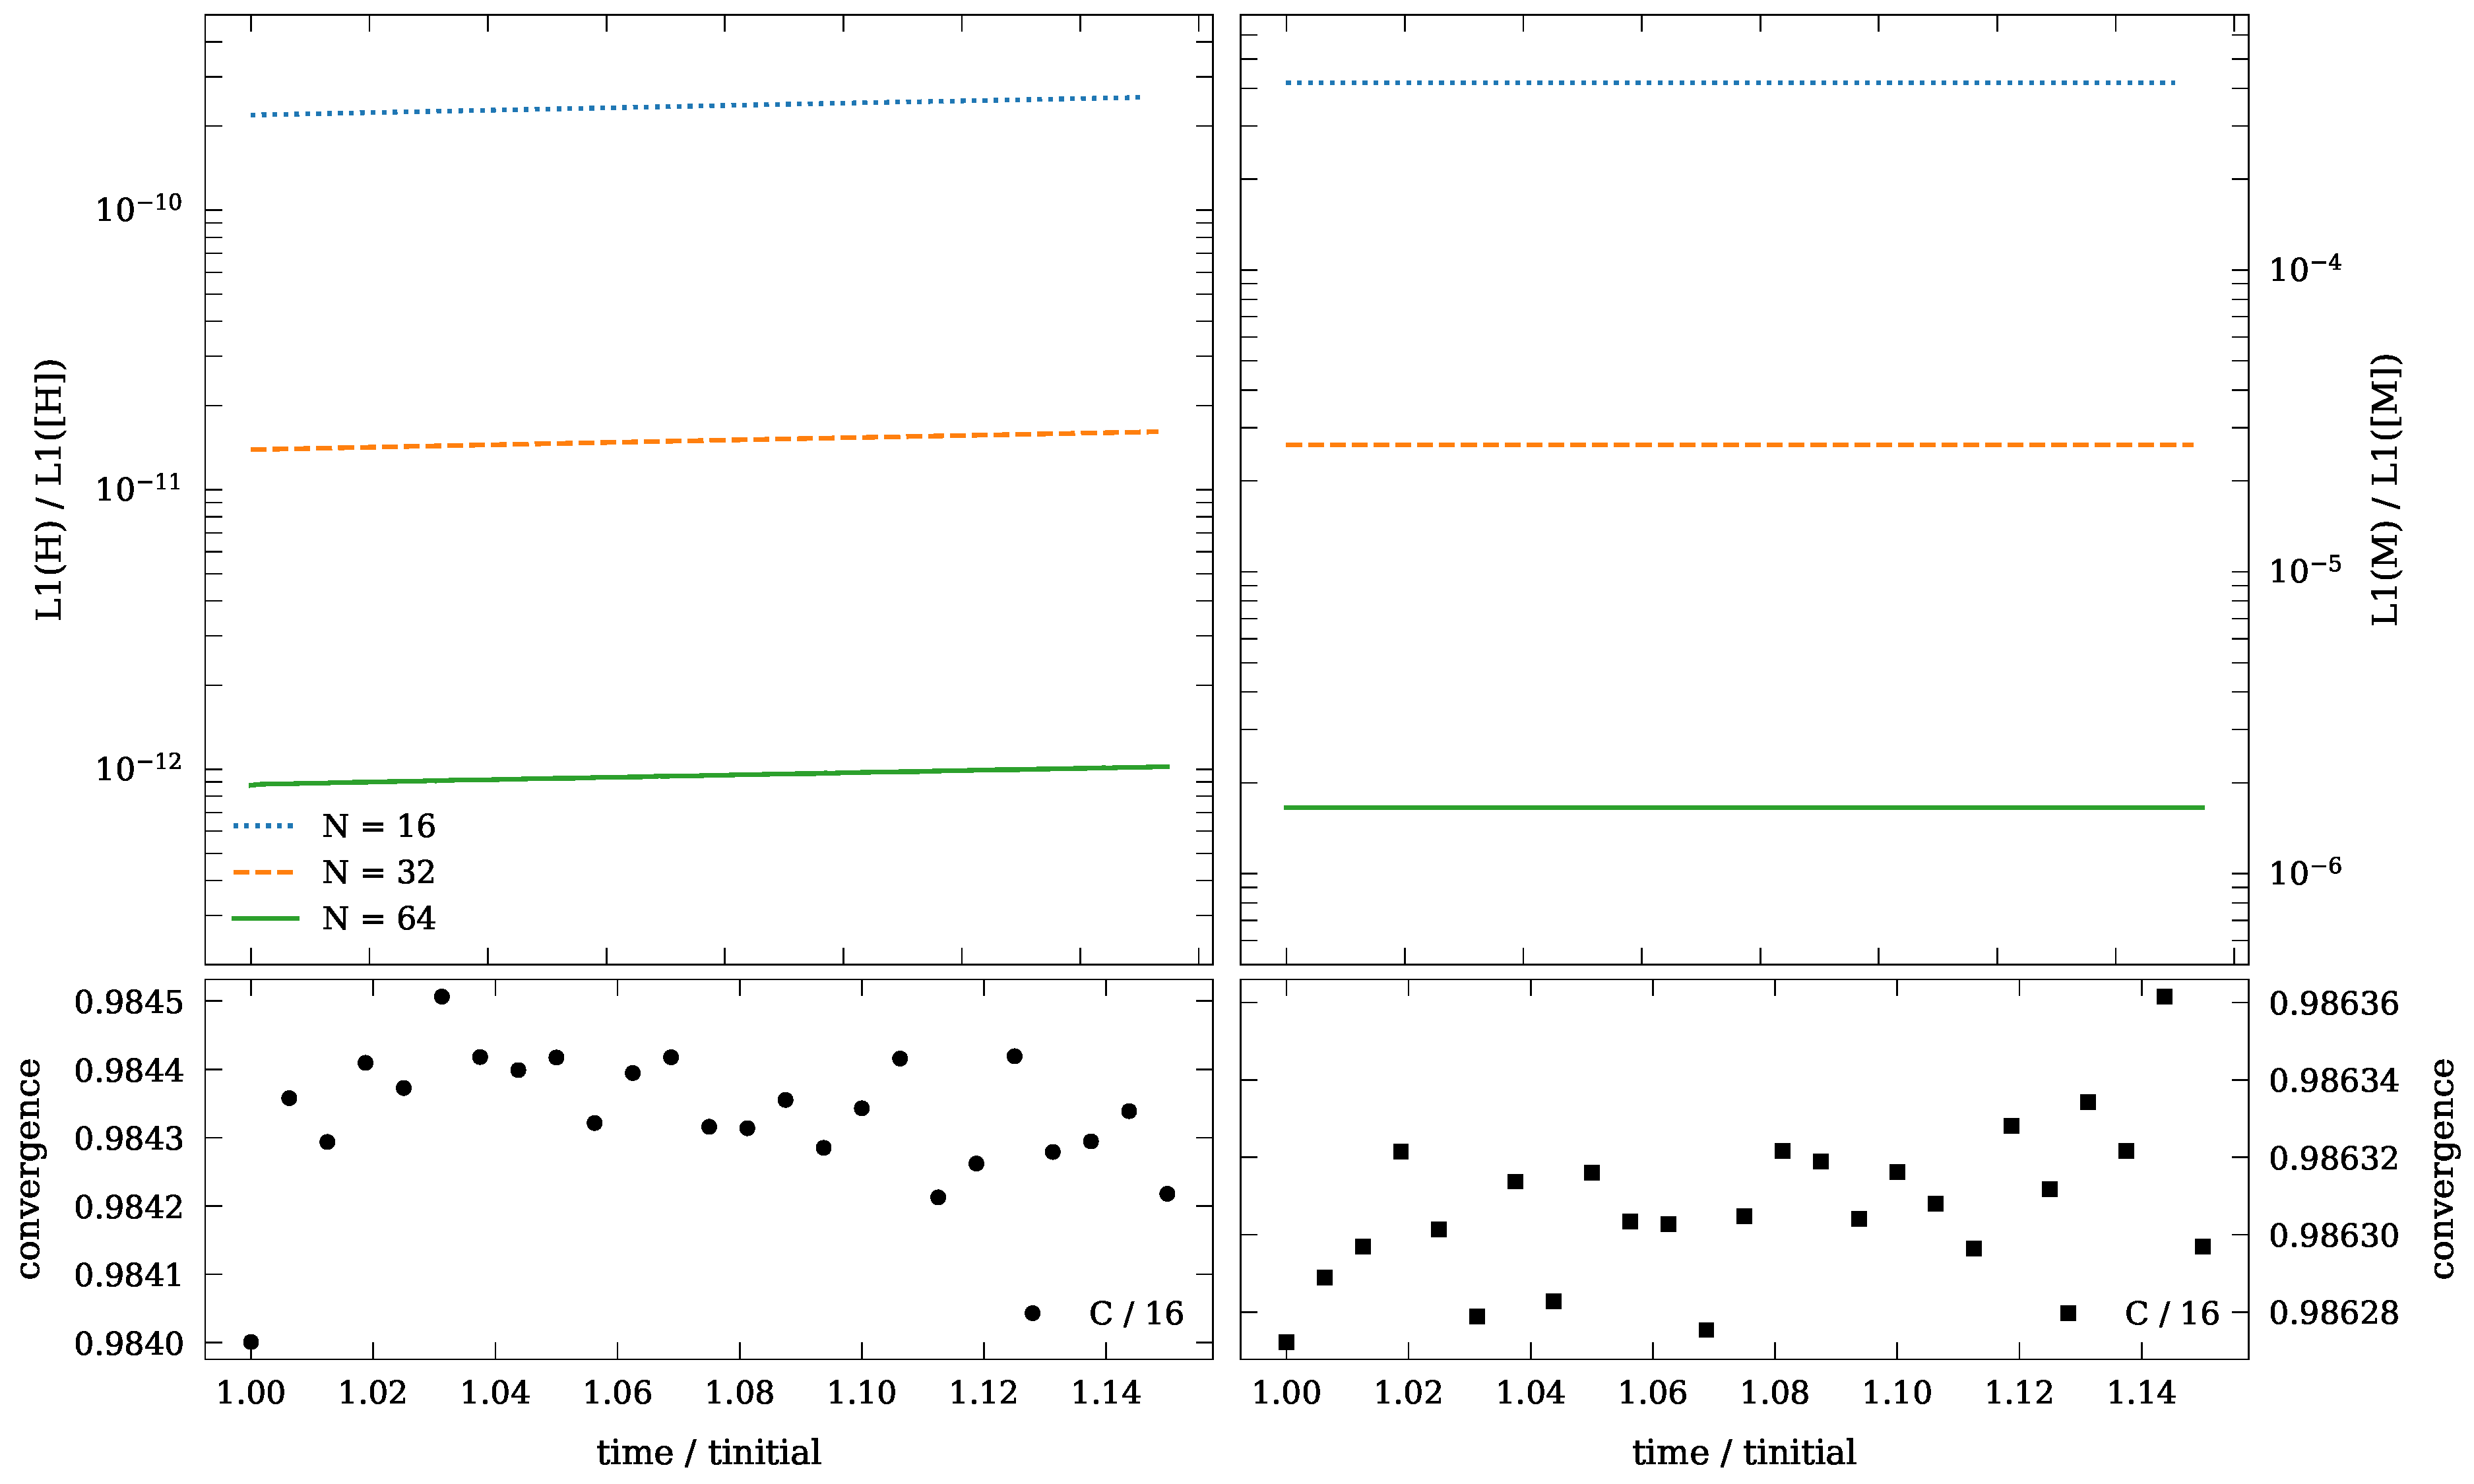
\includegraphics[width=0.8\textwidth]{figures/LinTest_Ham_Mom_rel_vs_time_16_32_64_wConvergence.pdf} 
	 %{figures/LinTest_Ham_Mom_rel_vs_time_16_32_64_wConvergence.pdf} 
  	 \caption{L1 error for the Hamiltonian (top left panel) and momentum (top right panel) constraint violations for the linear \mesc\, test with metric perturbation amplitude $\phi_0=10^{-8}$. We show three resolutions in each top panel vs time, and each bottom panel shows the respective convergence factor over time relative to the expected value; 16 for fourth order convergence.}
 	  \label{fig:Lintest_constraints_phi1em8}
\end{figure}

Figure~\ref{fig:Lintest_constraints_phi1em8} shows the time evolution of the Hamiltonian (top left panel) and momentum (top right panel) constraint violations for three resolutions $N=16,32,64$. Each violation is the L1 error normalised to the relevant ``energy scale'' \citep[see][]{macpherson2019b}. The respective bottom panels show the convergence factor \eqref{eq:convergence} for each time step, normalised to the expected value of 16 for fourth-order convergence. We see the expected convergence in the constraints as we increase resolution, and the violation remains constant as expected.

%
% No point showing linear solutions when we show 2nd order ones...
%
%\vspace{6mm}
%\textbf{\textit{Linearised analytic solutions}}
%\vspace{2mm}
%
%Here we study the errors between the \mesc\, calculations and the \emph{linearised solutions} for the Ricci scalar, expansion scalar, shear tensor component and shear scalar.
%We make sure to keep $\phi_0\ll1$ such that higher-order terms can safely be neglected. We study the errors for the second-order solutions in the next section, with slightly larger perturbation sizes. 
%
%%%%%%%% multi-panel figure
%\begin{figure}
%    \begin{subfigure}{.5\textwidth}
%          \centering
%          \includegraphics[width=0.97\linewidth]{../testruns/notebooks/plots/Linear_Analytic_Solns/Lintest_convergence_N16_32_64_phi1em8_allvars.pdf}
%     %     \caption{}
%       %   \label{fig:Lintest_convergence_phi1em8}
%    \end{subfigure}%
%    \begin{subfigure}{.5\textwidth}
%          \centering
%          \includegraphics[width=0.97\linewidth]{../testruns/notebooks/plots/Linear_Analytic_Solns/Lintest_convergence_N32_64_128_phi1em8_allvars_not_trR.pdf}
% %         \caption{}
%       %   \label{fig:Lintest_convergence_highres_phi1em8}
%    \end{subfigure}
%    \caption{Convergence rate \eqref{eq:convergence} of the relative error between \mesc\, calculations and linearised analytic variables (as indicated in the legend) for a metric perturbation with $\phi_0=10^{-8}$. In the left panel we use resolutions $N = 16, 32$, and $64$ to calculate $C$, and in the right panel we use $N = 32$, $64$, and $128$. In the right panel we have omitted ${}^{(3)}R$ since at $N=128$ the error reaches roundoff error, and so does not converge. The dashed line shows the expected fourth-order convergence, i.e. $C=16$.}
%    \label{fig:LinTest_Convergence}
%\end{figure}
%
%The left panel of Figure~\ref{fig:LinTest_Convergence} shows the convergence rate for the normalised L1 error \eqref{eq:L1normalised} using three different spatial resolutions $N = 16, 32$, and $64$, for a metric perturbation with amplitude $\phi_0=10^{-8}$. The $x$-axis shows 25 iterations (for the lowest resolution, which corresponds to double and quadruple this number of iterations for the medium and higher resolution, respectively), since the calculations themselves require time derivatives. The right panel of Figure~\ref{fig:LinTest_Convergence}  is the same as the left but with higher resolutions $N = 32, 64$, and $128$. We have omitted ${}^{(3)}R$ in this panel, since for $N=128$, the error has reached roundoff and so does not converge. The dashed line in both panels shows the expected fourth-order convergence.
%
%The convergence rate improves as we increase the resolution (moving from left to right panels of Figure~\ref{fig:LinTest_Convergence}), and is extremely close to the expected fourth-order convergence. The convergence rate is unaffected by the perturbation amplitude $\phi_0$, as we have tested for $\phi_0=10^{-8}, 10^{-10},$ and $10^{-12}$ (all regimes within which we expect a match with the linear solution). We do not find convergence when using $\phi_0=10^{-5}$ since in this regime we expect higher-order terms to become important, and so the linear solution is not sufficient. We compare the \mesc\, results to second-order solutions in the following section. 
%
%\begin{figure}[h]
%	\centering
%  	 \includegraphics[width=0.8\textwidth]{../testruns/notebooks/plots/Linear_Analytic_Solns/Lintest_L1error_N64_AllPhi_AllVars.pdf} 
%  	 \caption{Normalised L1 error for four different variables calculated in \mesc\, vs. the linearised analytic solutions. All errors are for an $N=64$ test with metric perturbation of different amplitudes (different curve styles, as indicated in the legend).}
% 	  \label{fig:Lintest_L1error}
%\end{figure}
%
%Figure~\ref{fig:Lintest_L1error} shows the normalised L1 error as a function of iteration for all variables studied here at resolution $N=64$. Different line styles represent different metric perturbation amplitudes $\phi_0$. We see the error relative to the linear solution reduce with perturbation size, as expected, for all variables except the Ricci scalar (bottom right panel). In this case, reducing the perturbation from $10^{-10}$ to $10^{-12}$ makes no difference to the error. The reason for this is that with such a small perturbation, the spacetime is extremely close to being flat. The Ricci scalar is simply spatial derivatives of the metric, and so these fall below roundoff error for a perturbation this small. 

%\vspace{6mm}
%\textbf{\textit{Second-order analytic solutions}}
%\vspace{2mm}

%Here we study the errors and convergence between the \mesc\, calculations and the second-order solutions for the expansion scalar, shear tensor component, and shear scalar. We use the full form of the Ricci scalar here.

%%%%%%% multi-panel figure
\begin{figure}[h!]
    \begin{subfigure}{.5\textwidth}
          \centering
          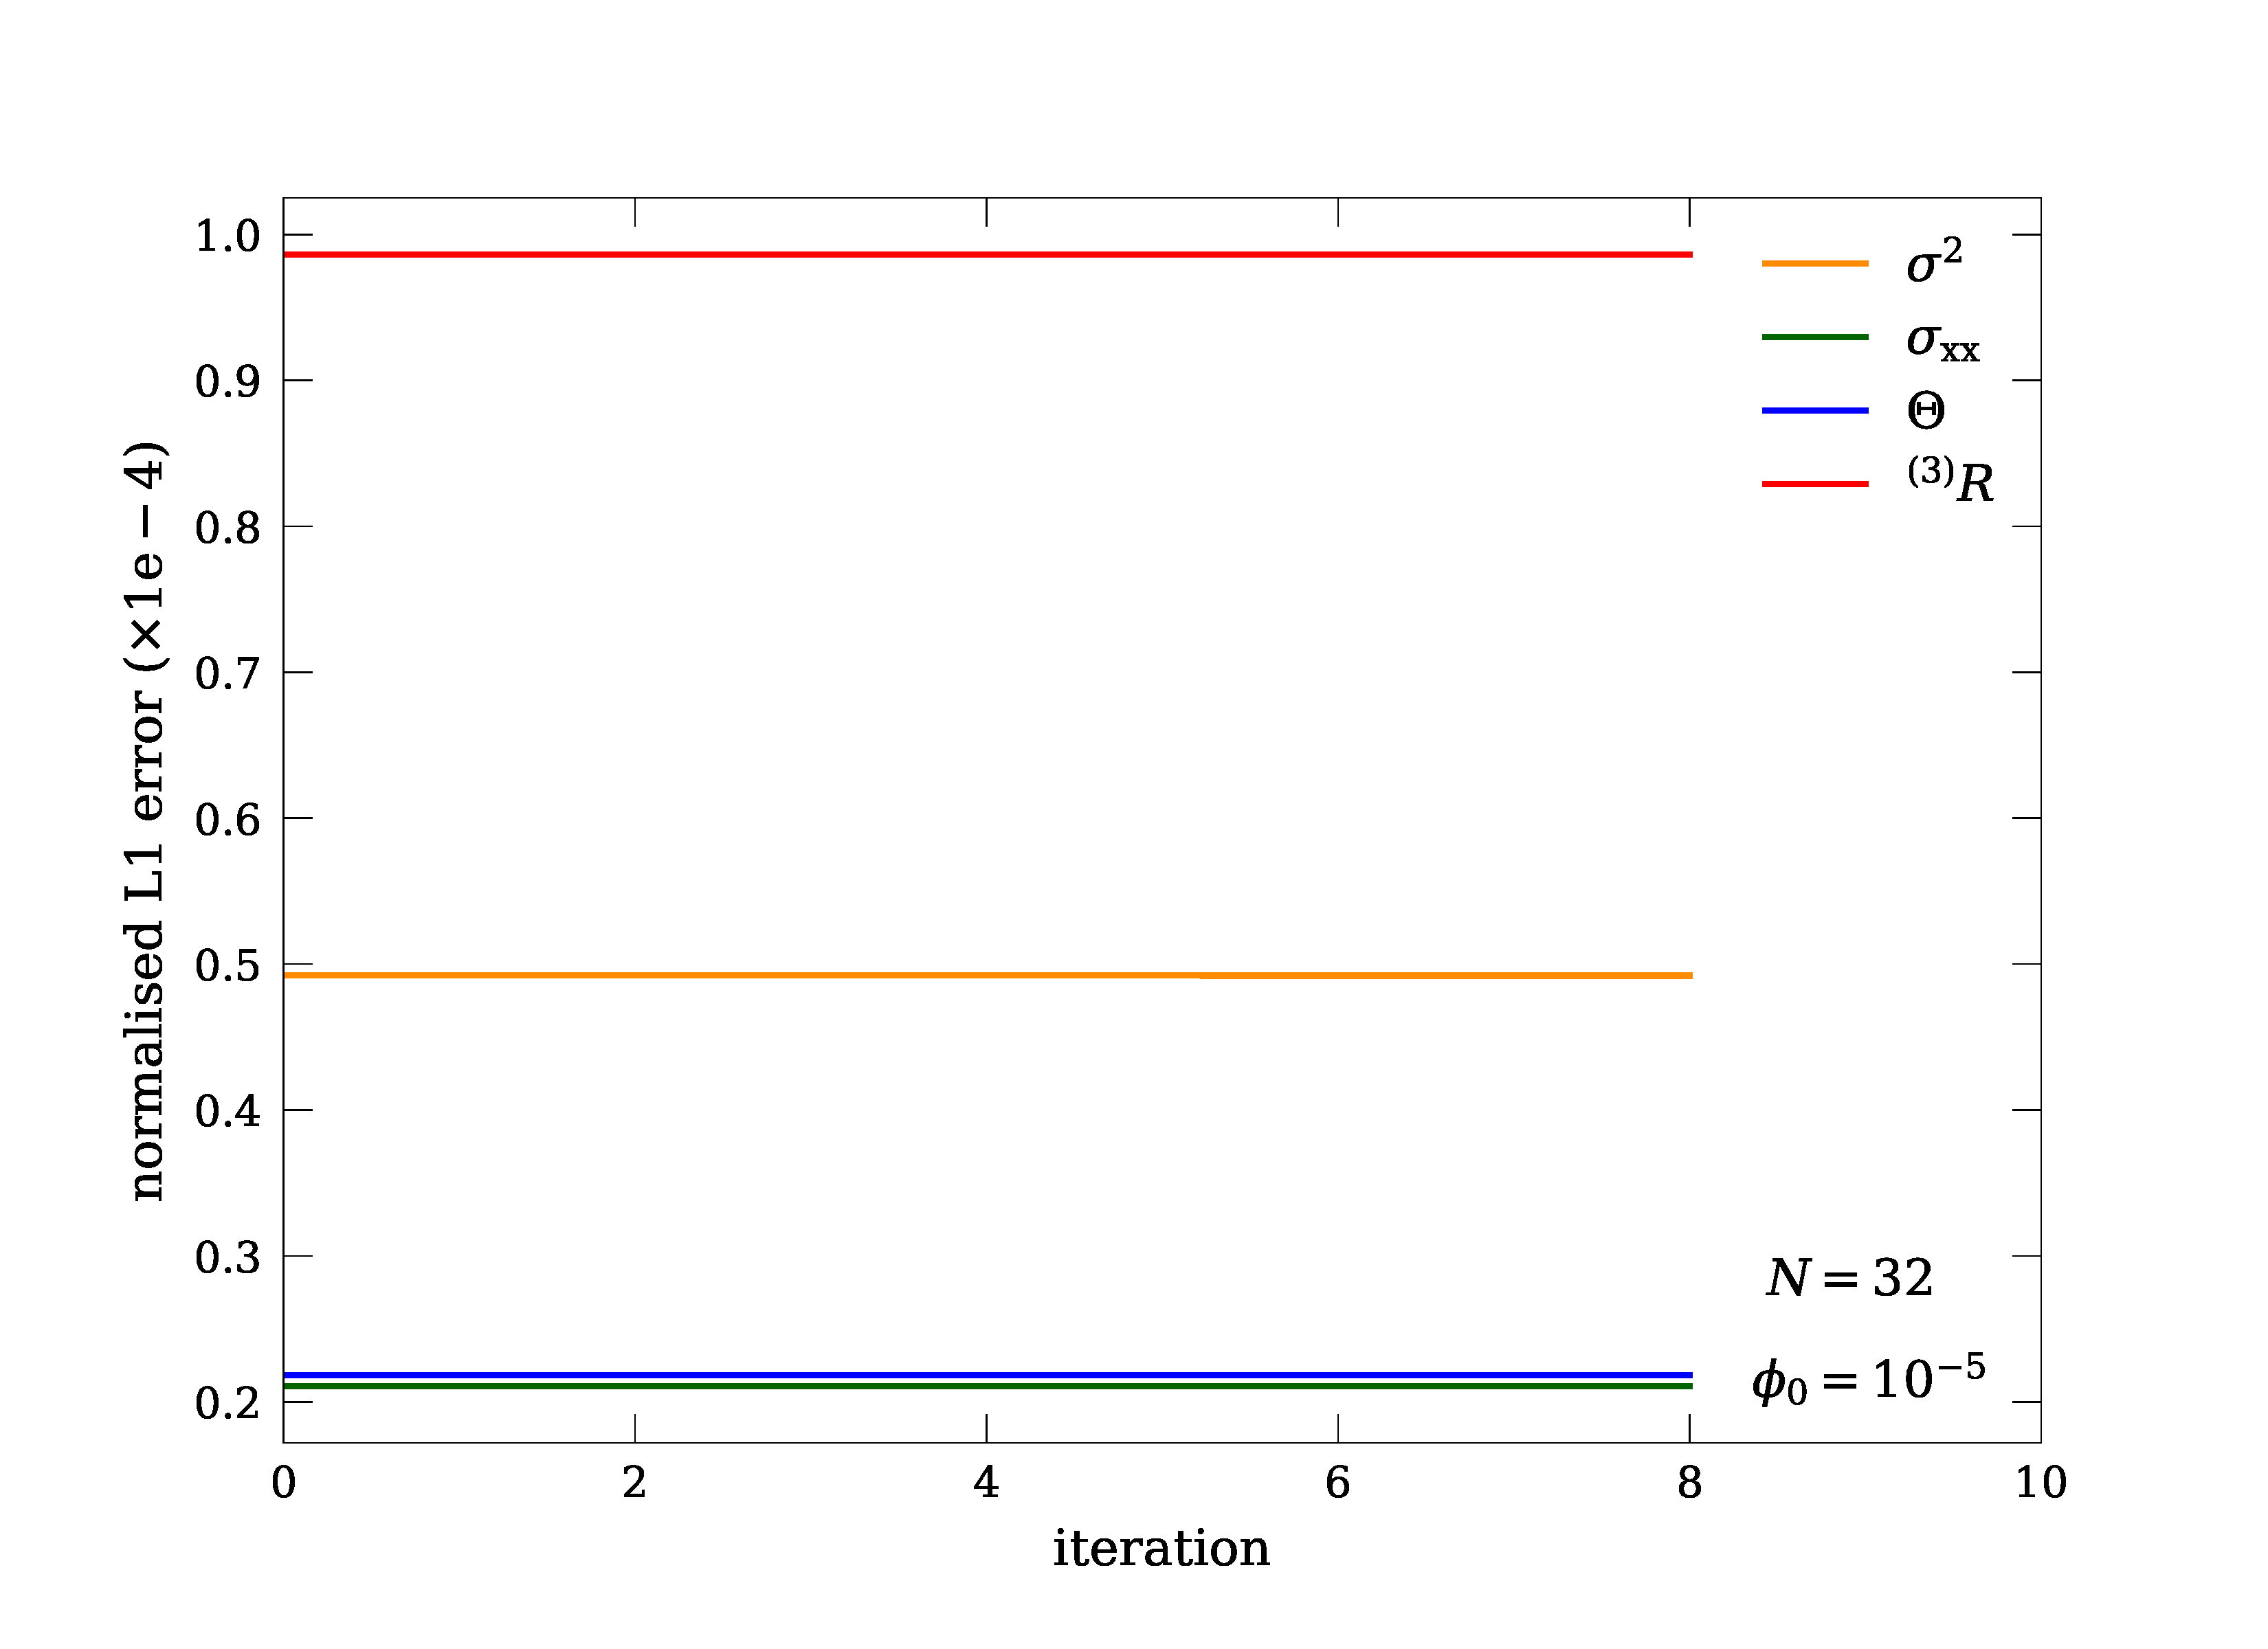
\includegraphics[width=\linewidth]{figures/LinPerturb_normedL1error_N32_amp1em5_allvars.pdf}
    \end{subfigure}%
    \begin{subfigure}{.5\textwidth}
          \centering
          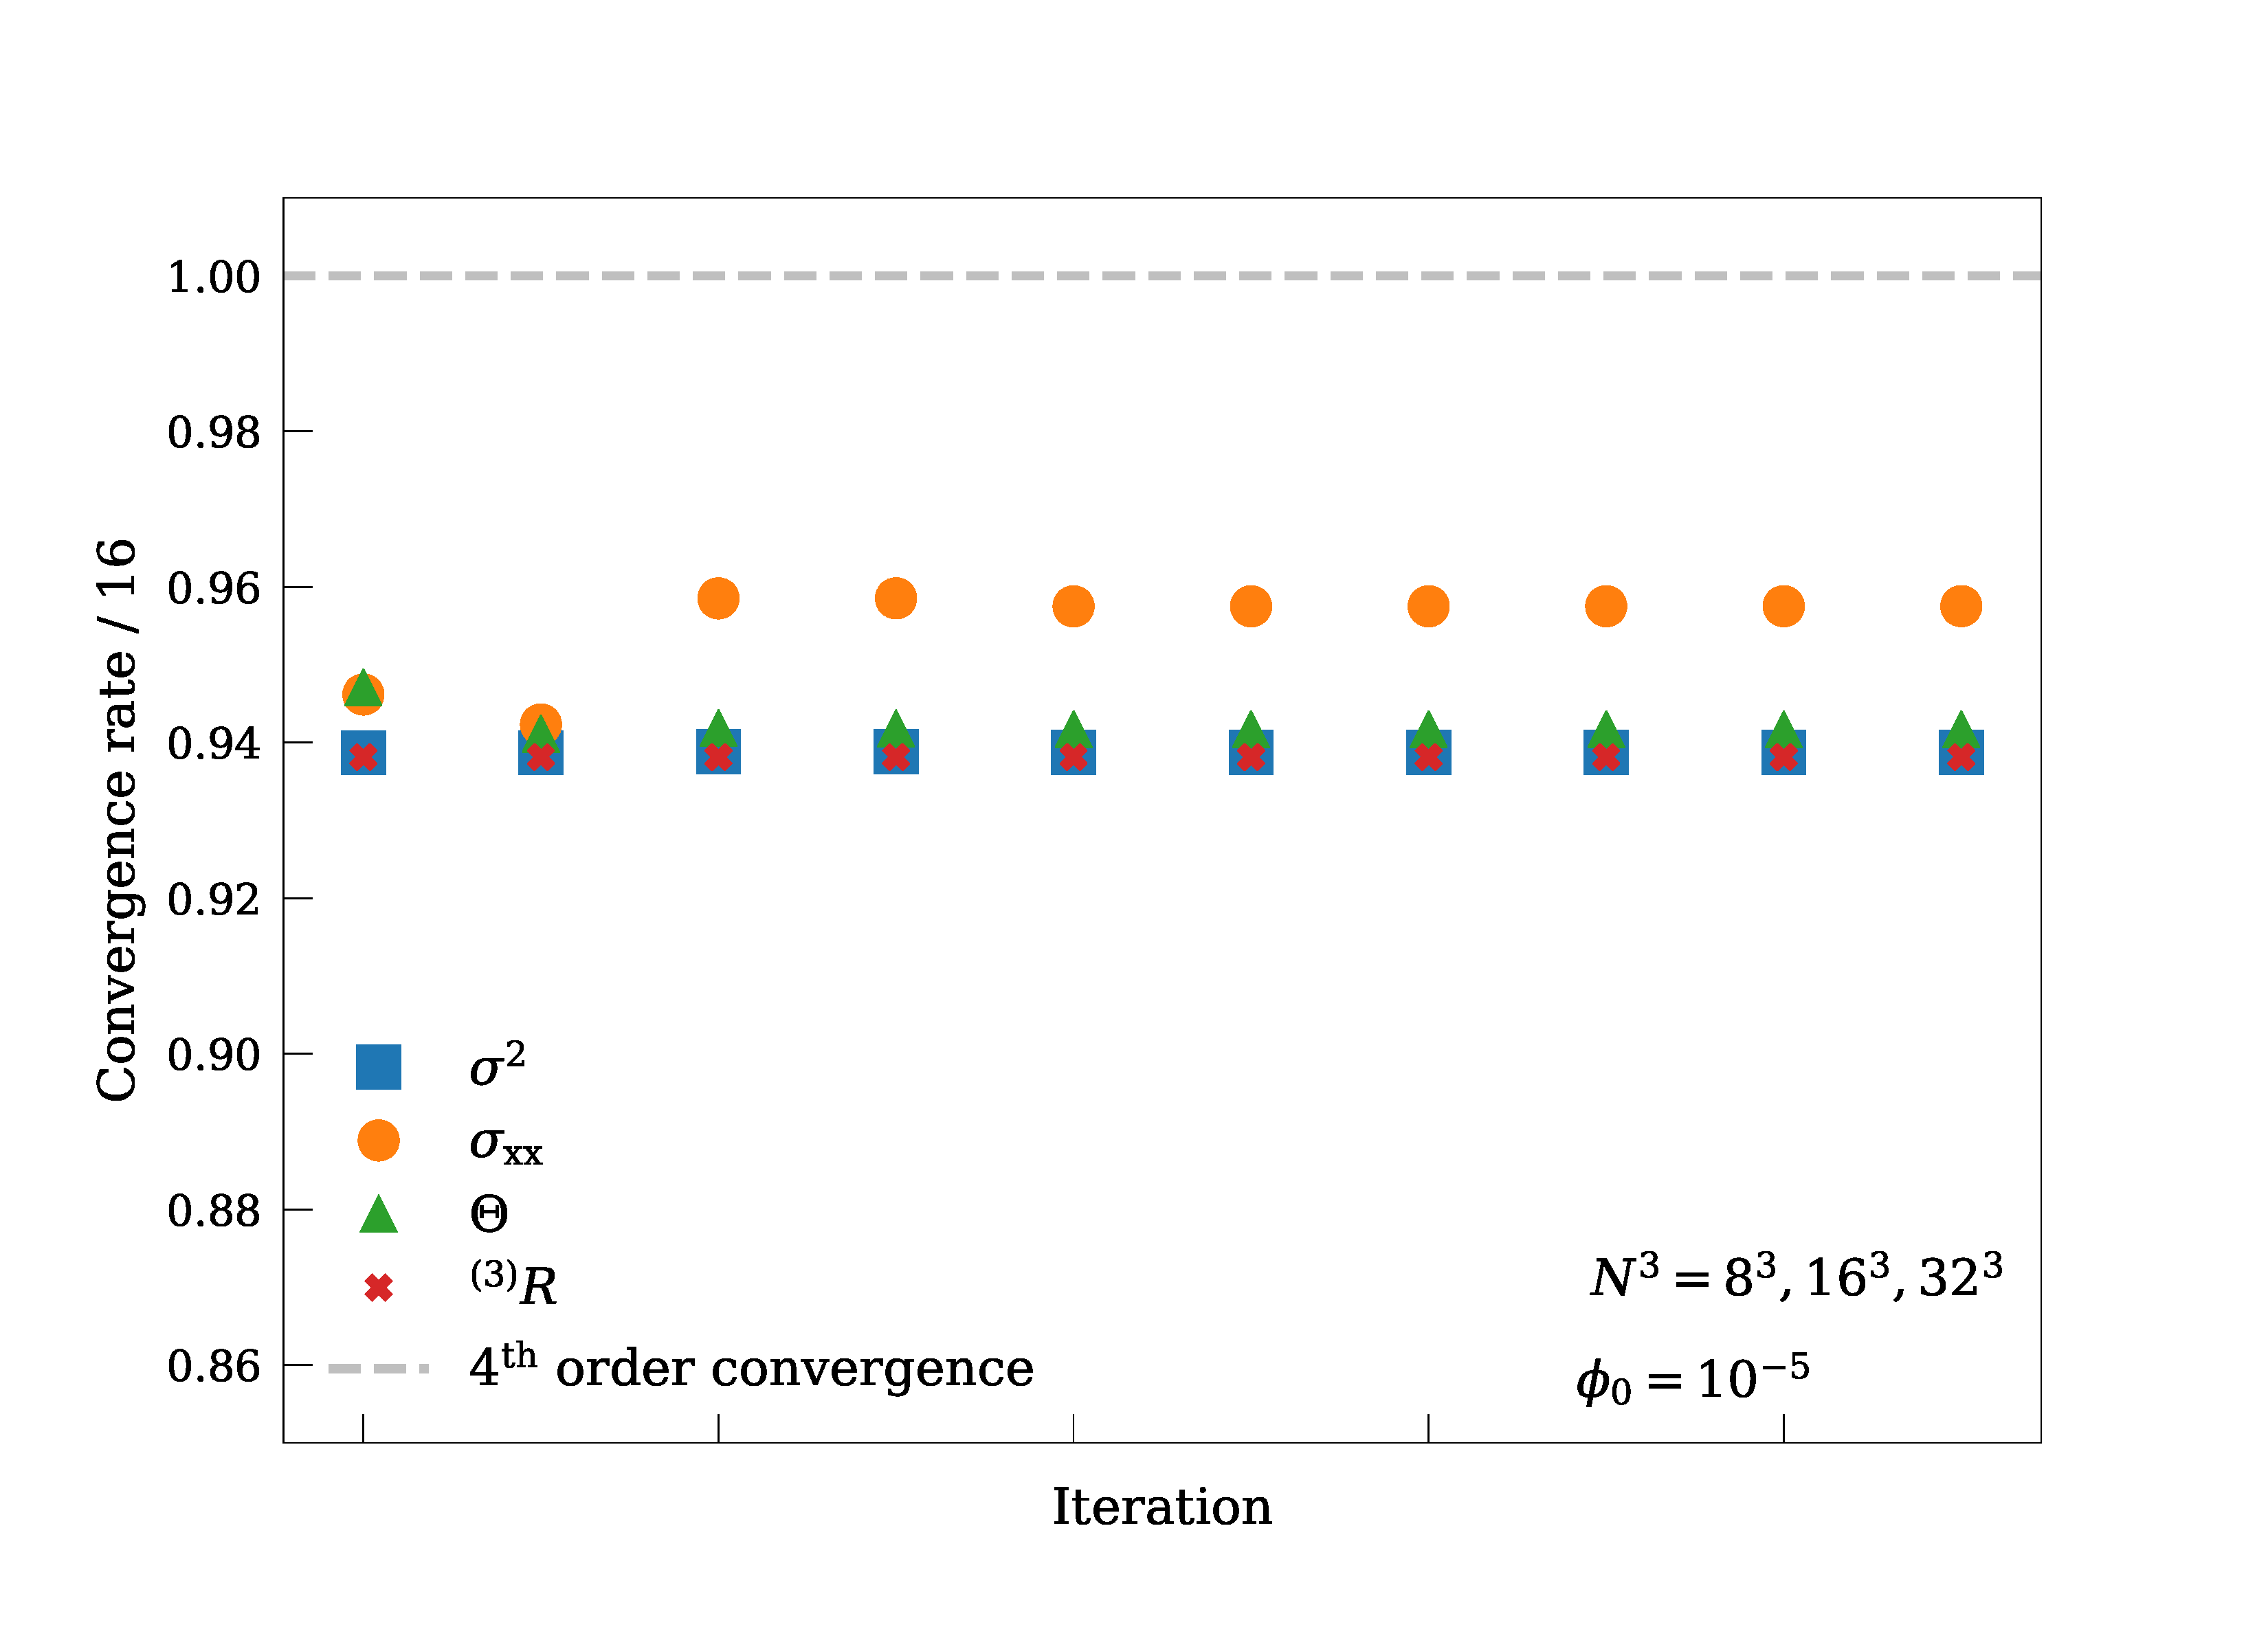
\includegraphics[width=\linewidth]{figures/Lintest_2ndorder_convergence_N8_16_32_phi1em5_allvars.pdf}
    \end{subfigure}
    \caption{Normalised L1 error (left panel) and convergence rate (right panel) for the second-order analytic solutions (full solution for the Ricci scalar) for the linearly-perturbed FLRW test. We show three resolutions $N=8,16$, and $32$ for a perturbation amplitude $\phi_0=10^{-5}$.}
    \label{fig:2ndorder_conv_phi1em5}
\end{figure}

The left panel of Figure~\ref{fig:2ndorder_conv_phi1em5}  shows the normalised L1 error for the expansion scalar, shear tensor, shear scalar and Ricci curvature for resolution $N=32$ and perturbation amplitude $\phi_0=10^{-5}$. The right panel shows the corresponding convergence rate for resolutions $N=8,16, 32$. At these resolutions, the convergence is independent of amplitude for all those we tested, specifically $\phi_0 = 10^{-12}, 10^{-10}, 10^{-8}, 10^{-5}$, and $10^{-3}$. At higher resolutions, the results for the kinematical variables do not converge as expected. This is most likely because at $N=64$ and above the numerical error falls below the error due to third order (and higher) contributions neglected in the analytic solutions. In the next section we study a non-perturbative solution and show that in that case, these variables converge at all resolutions studied.

%%%%%%% multi-panel figure
\begin{figure}[h!]
    \begin{subfigure}{.5\textwidth}
          \centering
          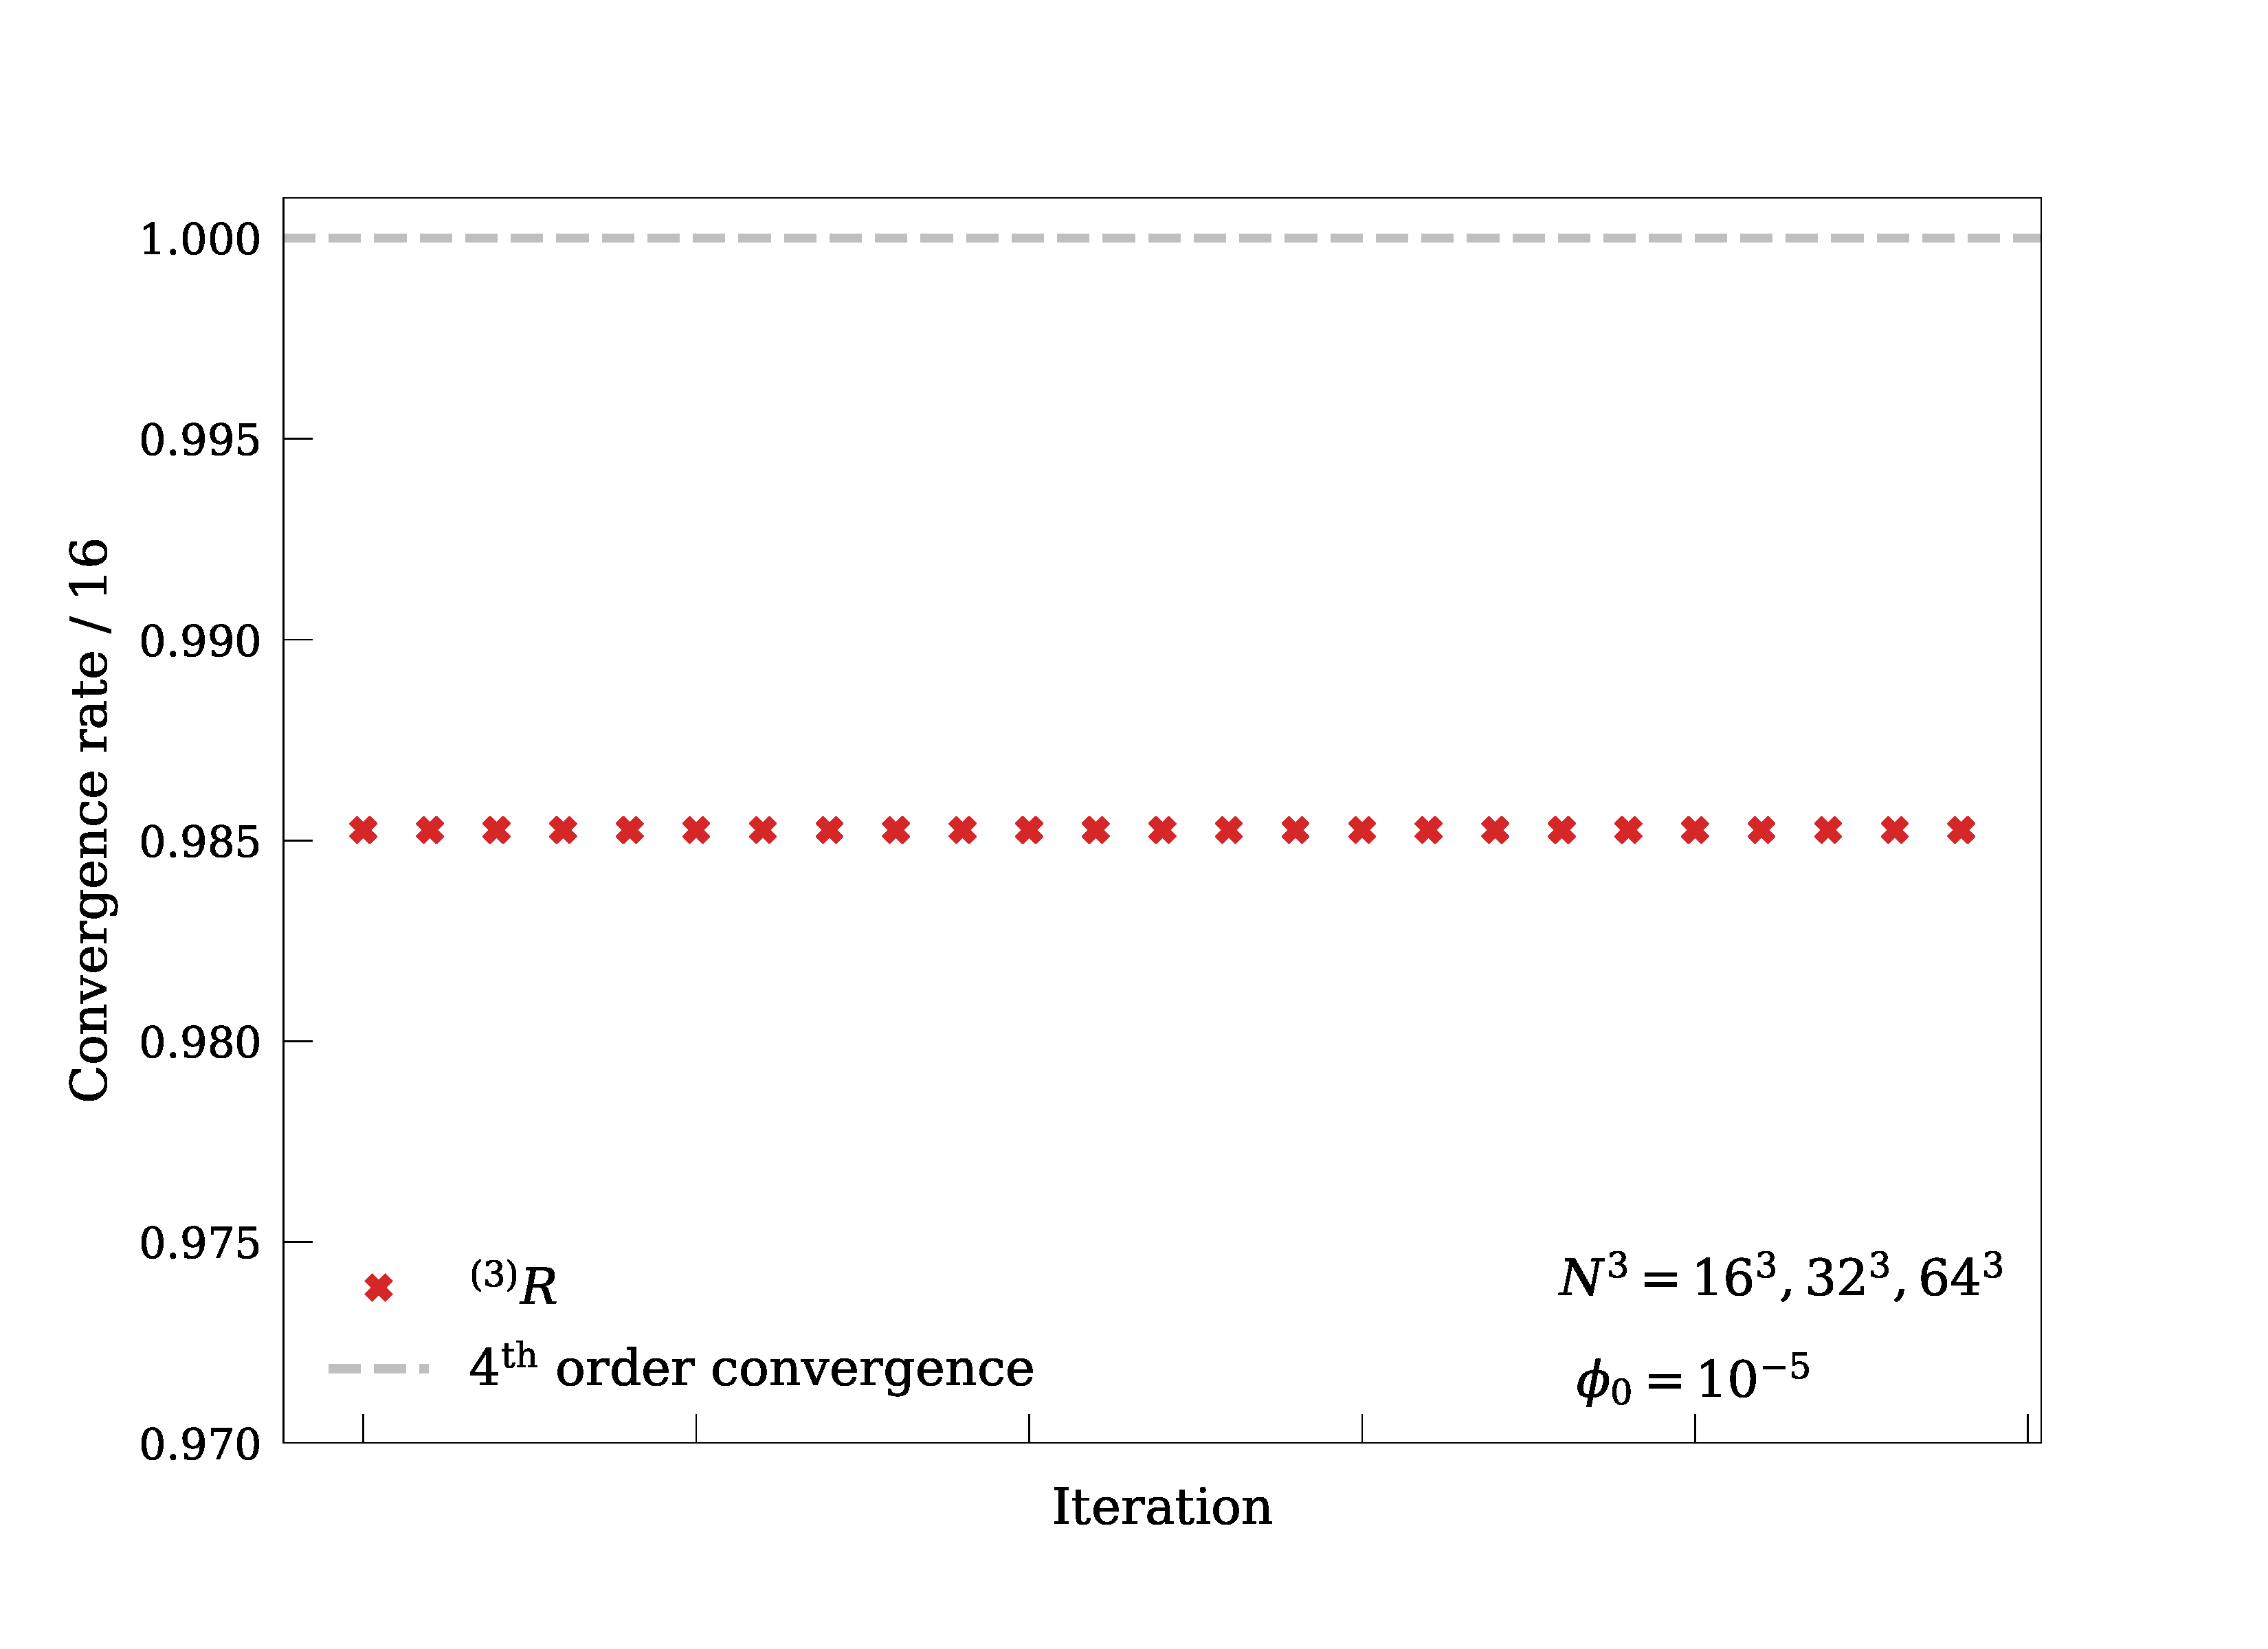
\includegraphics[width=0.97\linewidth]{figures/Lintest_2ndOrderAnalytic_convergence_N16_32_64_phi1em5_onlytrR.pdf}
    \end{subfigure}%
    \begin{subfigure}{.5\textwidth}
          \centering
          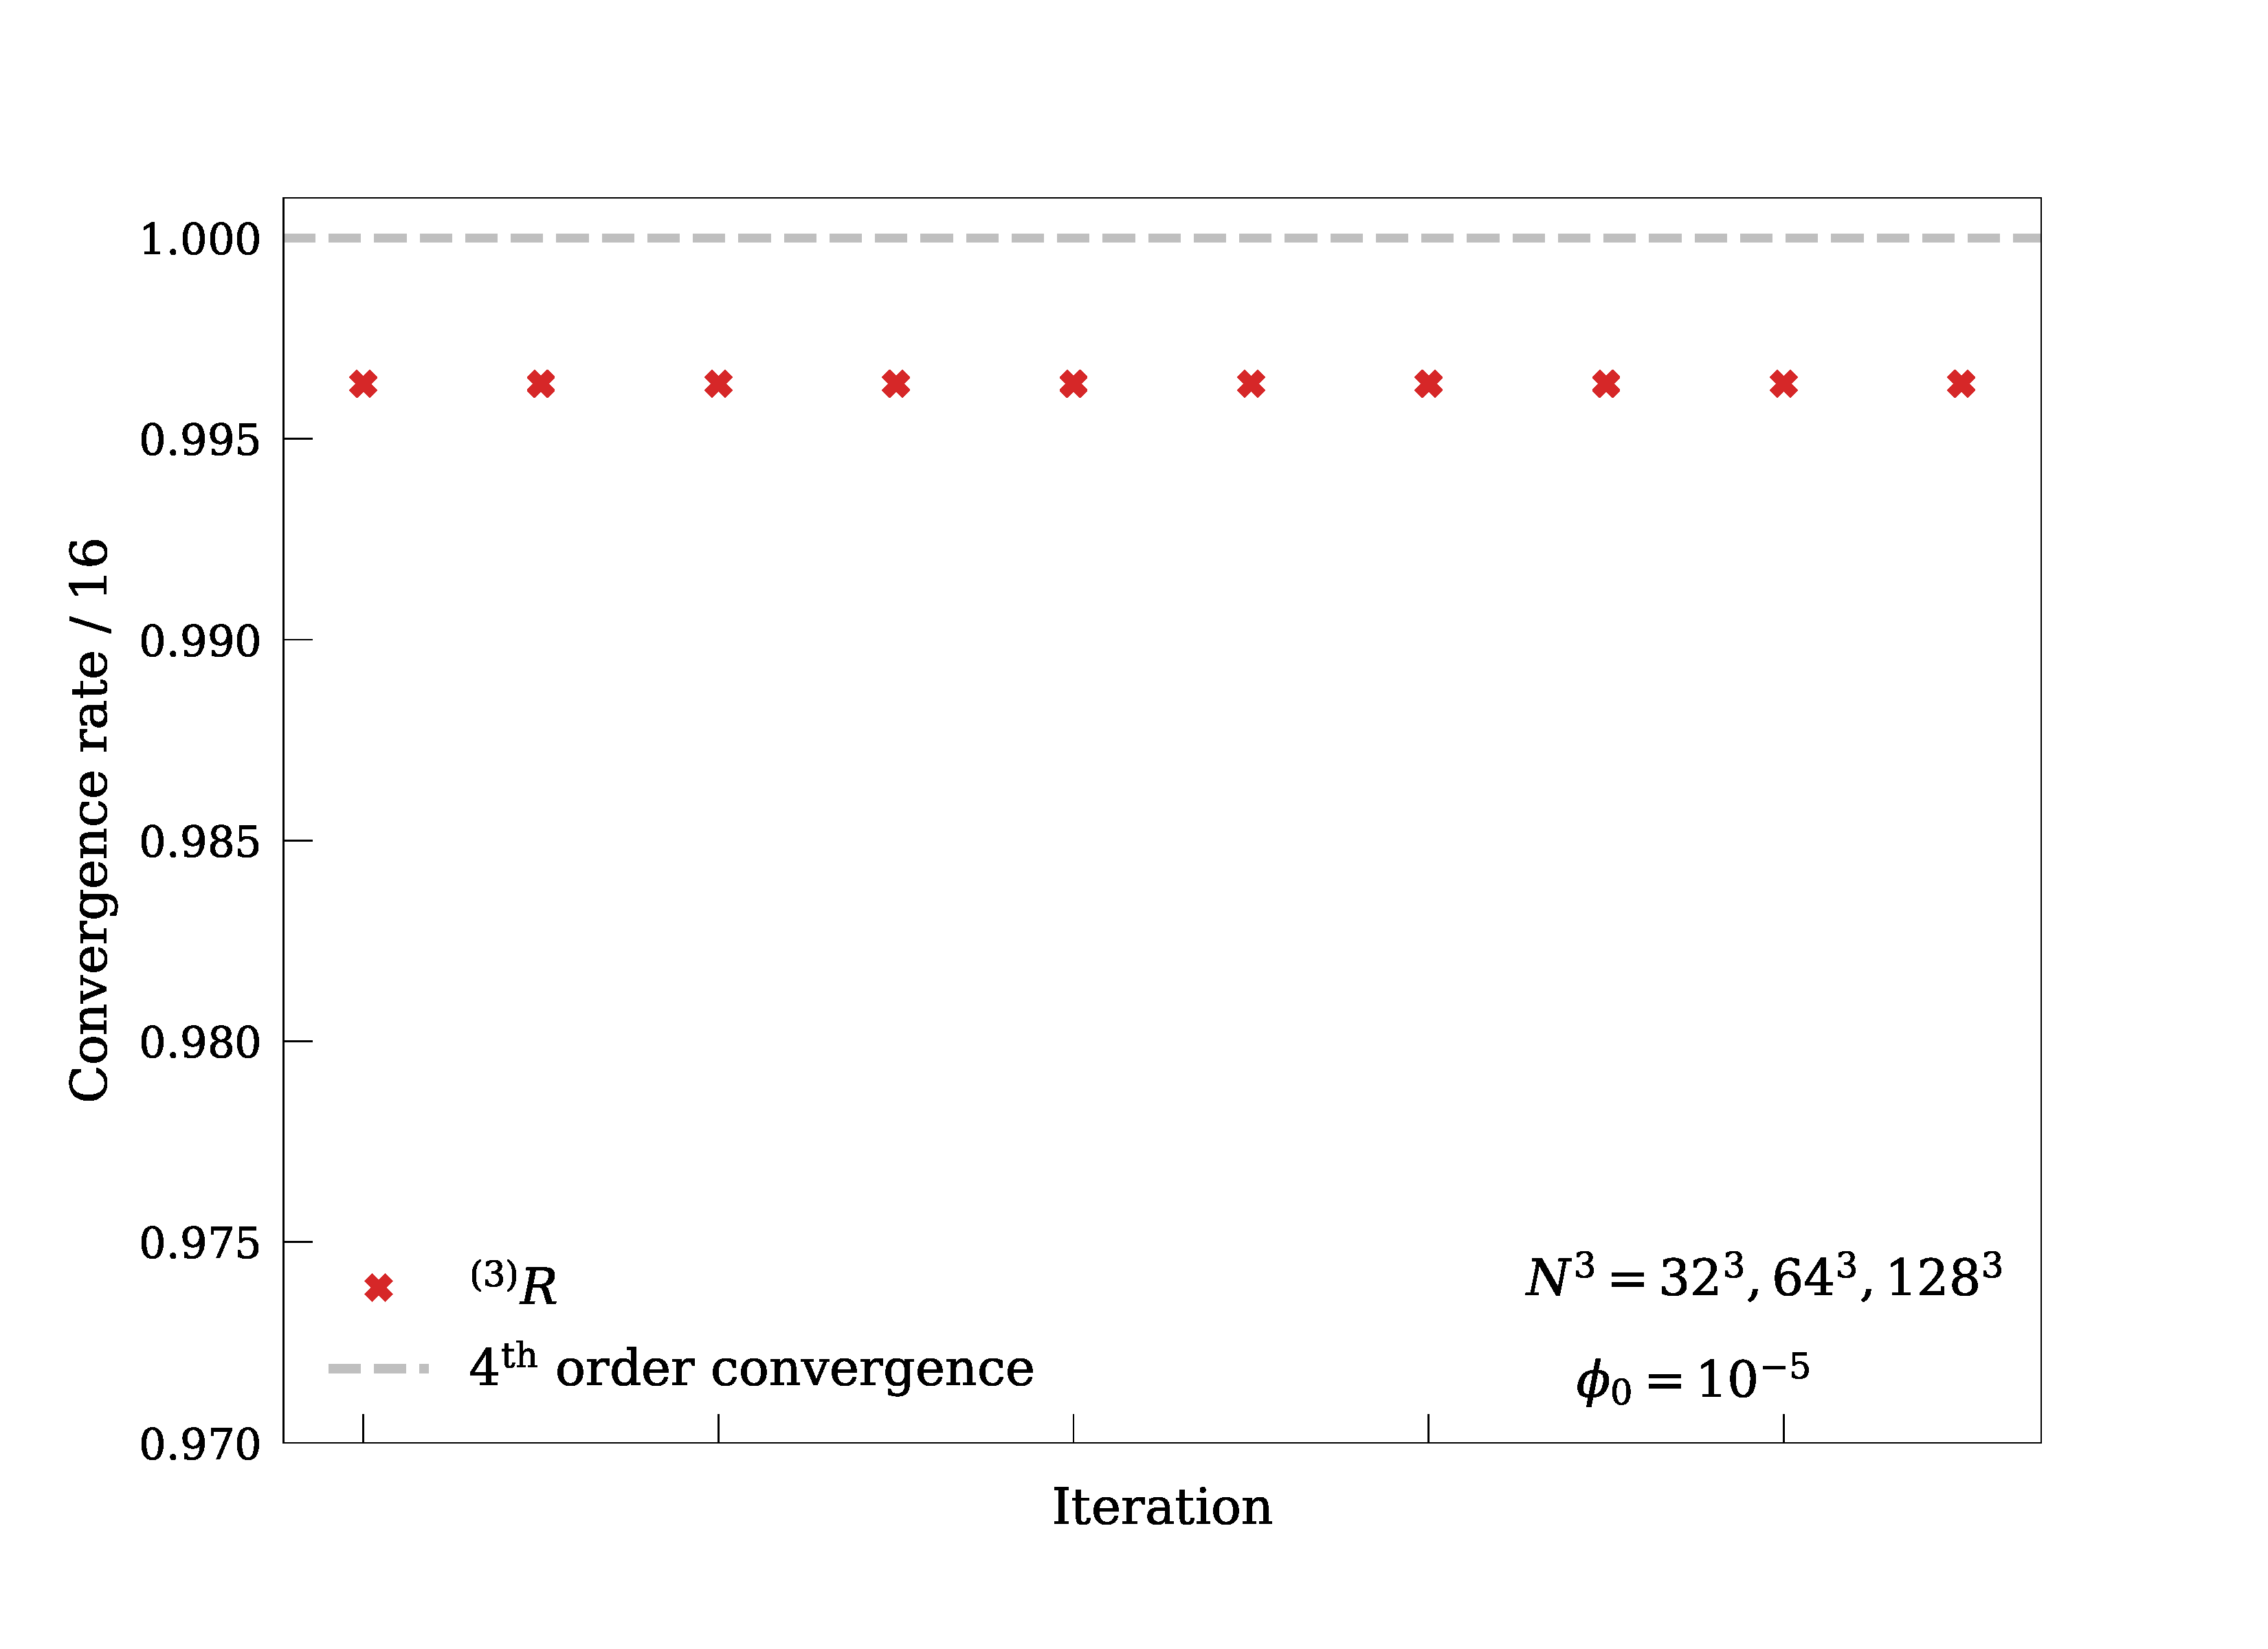
\includegraphics[width=0.97\linewidth]{figures/Lintest_2ndOrderAnalytic_convergence_N32_64_128_phi1em5_onlytrR.pdf}
    \end{subfigure}
    \caption{Convergence rate \eqref{eq:convergence} of the relative error between the \mesc\, calculation of the Ricci scalar and full analytic solution for a metric perturbation with $\phi_0=10^{-5}$. In the left panel we use resolutions $N = 16, 32$, and $64$ to calculate $C$, and in the right panel we use $N = 32$, $64$, and $128$. The dashed line shows the expected fourth-order convergence, i.e. $C=16$.}
    \label{fig:LinTest_2ndorder_3RConvergence}
\end{figure}

The analytic solution for Ricci scalar used here is non-perturbative, and so the error is purely numerical. In Figure~\ref{fig:LinTest_2ndorder_3RConvergence} we show the convergence rate for ${}^{(3)}R$ for $N=16,32,64$ (left panel) and $N=32,64,128$ (right panel), for a perturbation with amplitude $\phi_0=10^{-5}$. We see an improvement in convergence with the increase in resolution.

\begin{figure}[h!]
	\centering
  	 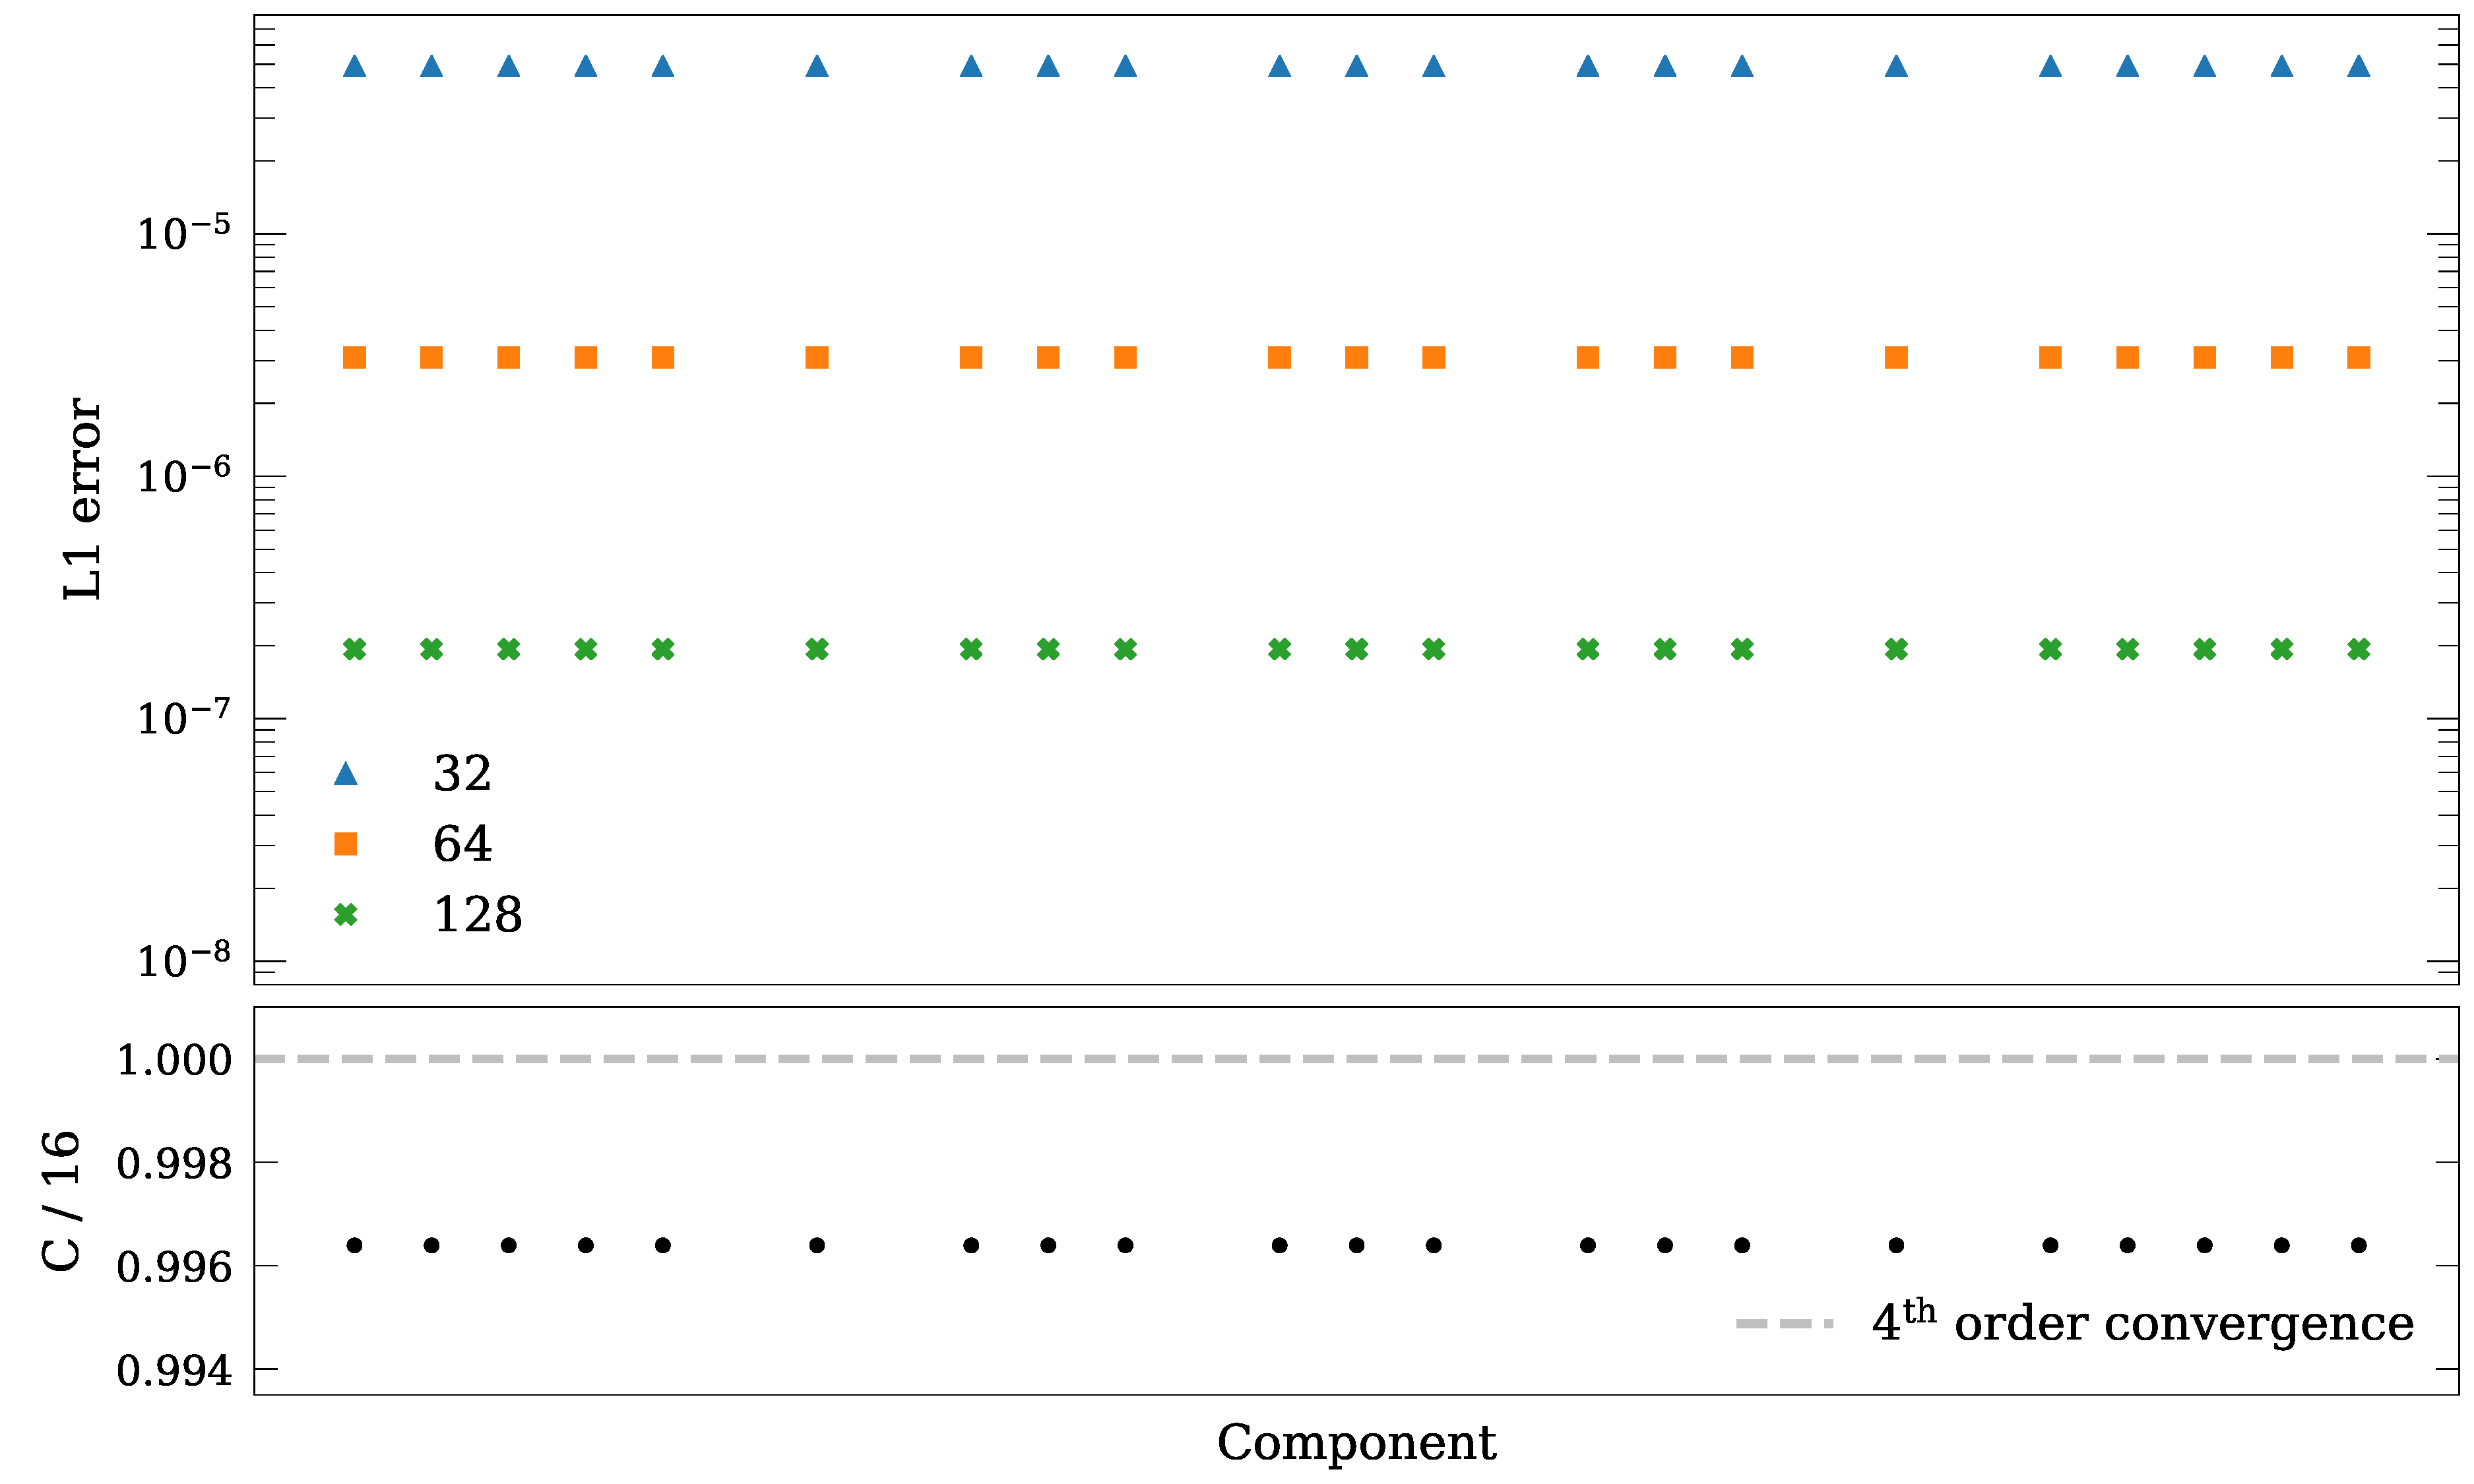
\includegraphics[width=0.7\textwidth]{figures/Lintest_2ndOrderAnalytic_L1_AND_convergence_N32_64_128_phi1em5_Christoffels.pdf} 
  	 \caption{Normalised L1 error (top panel) and convergence rate (bottom panel) for all 27 components of the spatial Christoffel symbols for a perturbation with amplitude $\phi_0=10^{-5}$. The error is relative to the full analytic solution for the linear metric. We show resolutions $N=32,64,128$. The x-axis is the component of the Christoffel symbol, i.e., each point represents the error for a single component of $\Gamma^i_{jk}$ at the initial time. The missing points correspond to components that are identically zero analytically, for which the \mesc\, output is also identically zero.}
 	  \label{fig:2ndorder_conv_phi1em5_Chrs}
\end{figure}

In Figure~\ref{fig:2ndorder_conv_phi1em5_Chrs} we test our calculation of all 27 spatial Christoffel symbols in \mesc, for a perturbation with amplitude $\phi_0=10^{-5}$. The top panel shows the normalised L1 error for resolutions $N=32,64,128$, and the bottom panel shows the corresponding convergence factor, normalised to the expected value for fourth-order convergence. In both panels, the x-axis corresponds to the separate components. Each point represents the L1 error (and convergence) for an individual component at the initial time. We only calculate these at the initial time, since they are purely spatial and contain no time derivatives and do not evolve in time (since $\dot{\phi}=0$). The normalised L1 error is very small for the highest resolution, and all components converge at the expected rate. 



%------------------------------------------------------------------------------------------------------
\subsection{Arbitrary metric and four-velocity test}
%------------------------------------------------------------------------------------------------------

The calculation of $\Theta$, $\sigma_{\mu\nu}$, and $\omega_{\mu\nu}$ is purely kinematical, and so does not care about the dynamics, e.g. Einstein's equations or the geodesic equation. We can therefore test these calculations (in isolation of other parts of the code that do depend on the dynamics, e.g. constraint violation) by constructing an arbitrary metric and four-velocity vector, ensuring only that the normalisation condition $g_{\mu\nu} u^\mu u^\nu$ is satisfied. 

%%%%%%%%%%
\subsubsection{The metric}
%%%%%%%%%%%

We choose a metric with off-diagonal components such that we induce both a shear and a vorticity, namely
\begin{equation}
	ds^2 = - dt^2 + dx^2 + dy^2 + 2 F(t,x) dx dy + dz^2,
\end{equation}
i.e. $g_{xx}=g_{yy}=g_{zz}=1$, and $g_{xy}=g_{yx}=F(t,x)$ where $F$ is entirely arbitrary. The extrinsic curvature for this metric is
\begin{equation}
	K_{xy} = K_{yx} = - \frac{1}{2} F',
\end{equation}
where all other components are zero, and its trace is
\begin{equation}
	K = - \frac{F F'}{g},
\end{equation}
and the spatial Ricci scalar ${}^{(3)}R=0$.

We choose a temporary four-velocity
\begin{equation}
	U^\mu_{\rm temp} = \left(1, F(t,x), 0, 0\right),
\end{equation}
and calculate the four-velocity $u^\mu$ as the normalised version of this vector, i.e.,
\begin{equation}
	u^\mu = \frac{U^\mu_{\rm temp} }{\sqrt{-g_{\alpha\beta}U^\alpha_{\rm temp} U^\beta_{\rm temp}}}.
\end{equation}
This gives
\begin{equation}
	u^\mu = \left( \frac{1}{\sqrt{ -g }}, \frac{F}{\sqrt{ -g }}, 0, 0 \right),
\end{equation}
where $g=-1+ F^2$ is the determinant of $g_{\mu\nu}$.

We find the peculiar velocity (as defined in \texttt{HydroBase}, and assumed to be sent into \mesc) using (for zero shift)
\begin{equation}
	v^i = \frac{u^i}{\alpha u^0},
\end{equation}
with $\alpha=-1$ for this case. This gives
\begin{equation}
	v^i = (F, 0, 0).
\end{equation}

%%%%%%%%%%%%%%%%%%%%%%%%
\subsubsection{Analytic solutions}
%%%%%%%%%%%%%%%%%%%%%%%%

The expansion scalar is
\begin{equation}
	\Theta = \frac{\pd_x F}{\sqrt{-g}},
\end{equation}
and the (symmetric) shear tensor components we test here are
\begin{align}
	\sigma_{00} &= \frac{F^2 (2+F^2) \pd_x F + 3 F^3 F'}{3(-g)^{5/2}}, \\
	\sigma_{0x} &= - \frac{(F (2+F^2) \pd_x F + 3 F^2 F')}{3(-g)^{5/2}}, \\
	\sigma_{xx} &= \frac{(2+F^2) \pd_x F + 3 F F'}{3(-g)^{5/2}},
\end{align}
and the shear scalar is
\begin{align}
	\sigma^2 &= \frac{-12 F (1 + F^2) \pd_x(F) F' - 4 (\pd_x F)^2 (1 + F^2 + F^4) - 3(1+4F^2) (F')^2}{12\, g^3}.
\end{align}
The (anti-symmetric) vorticity tensor components are
\begin{align}
	\omega_{0y} &= \frac{F^2 (F F' + 2\pd_x F)}{2(-g)^{3/2}}, \\
	\omega_{xy} &= -\frac{F (F F' + 2\pd_x F)}{2(-g)^{3/2}}, \\
\end{align}
and the vorticity scalar is
\begin{equation}
	\omega^2 = - \frac{F^2 ( FF' + 2 \pd_x F)^2}{4 \, g^3}.
\end{equation}

The components of the four-acceleration tested here are
\begin{align}
	a^0 &= \frac{F(F\pd_x F + F')}{g^2}, \\
	a^x &= \frac{F \pd_x F + F'}{(-g)}.
\end{align}	
%and $\omega_{00}=\omega_{0x}=\omega_{0z}=\omega_{xx}=\omega_{yy}=\omega_{zz}=\omega_{zy}=\omega_{zx}=0$. 


%%%%%%%%%%%%%%%%%%%%%%%%
\subsubsection{Results}
%%%%%%%%%%%%%%%%%%%%%%%%

We choose the form of the function $F$ to be
\begin{equation}
	F(t,x) = F_0 \, t^{-2/3} \, {\rm sin}\left(\frac{2 \pi x}{L}\right)
\end{equation}
such that
\begin{align}
	\pd_x F &= \frac{2 \pi F_0 x}{L} \, t^{-2/3} \, {\rm cos}\left(\frac{2 \pi x}{L}\right), \\
		      F' &= -\frac{2 F_0}{3} \, t^{-5/3} \, {\rm sin}\left(\frac{2 \pi x}{L}\right),
\end{align}
where $F_0$ is an arbitrary amplitude, and $L$ is the box size, and we have assumed $t_{\rm init}>0$. We note that since the solution is non-perturbative, we do not require $F_0\ll 1$ for the analytic solutions above to be correct. We do, however, require $|F_0|<1$ (at the initial time) so that $|v^i| < c$.

%%%%%%% multi-panel figure
\begin{figure}[h!]
    \begin{subfigure}{.5\textwidth}
          \centering
          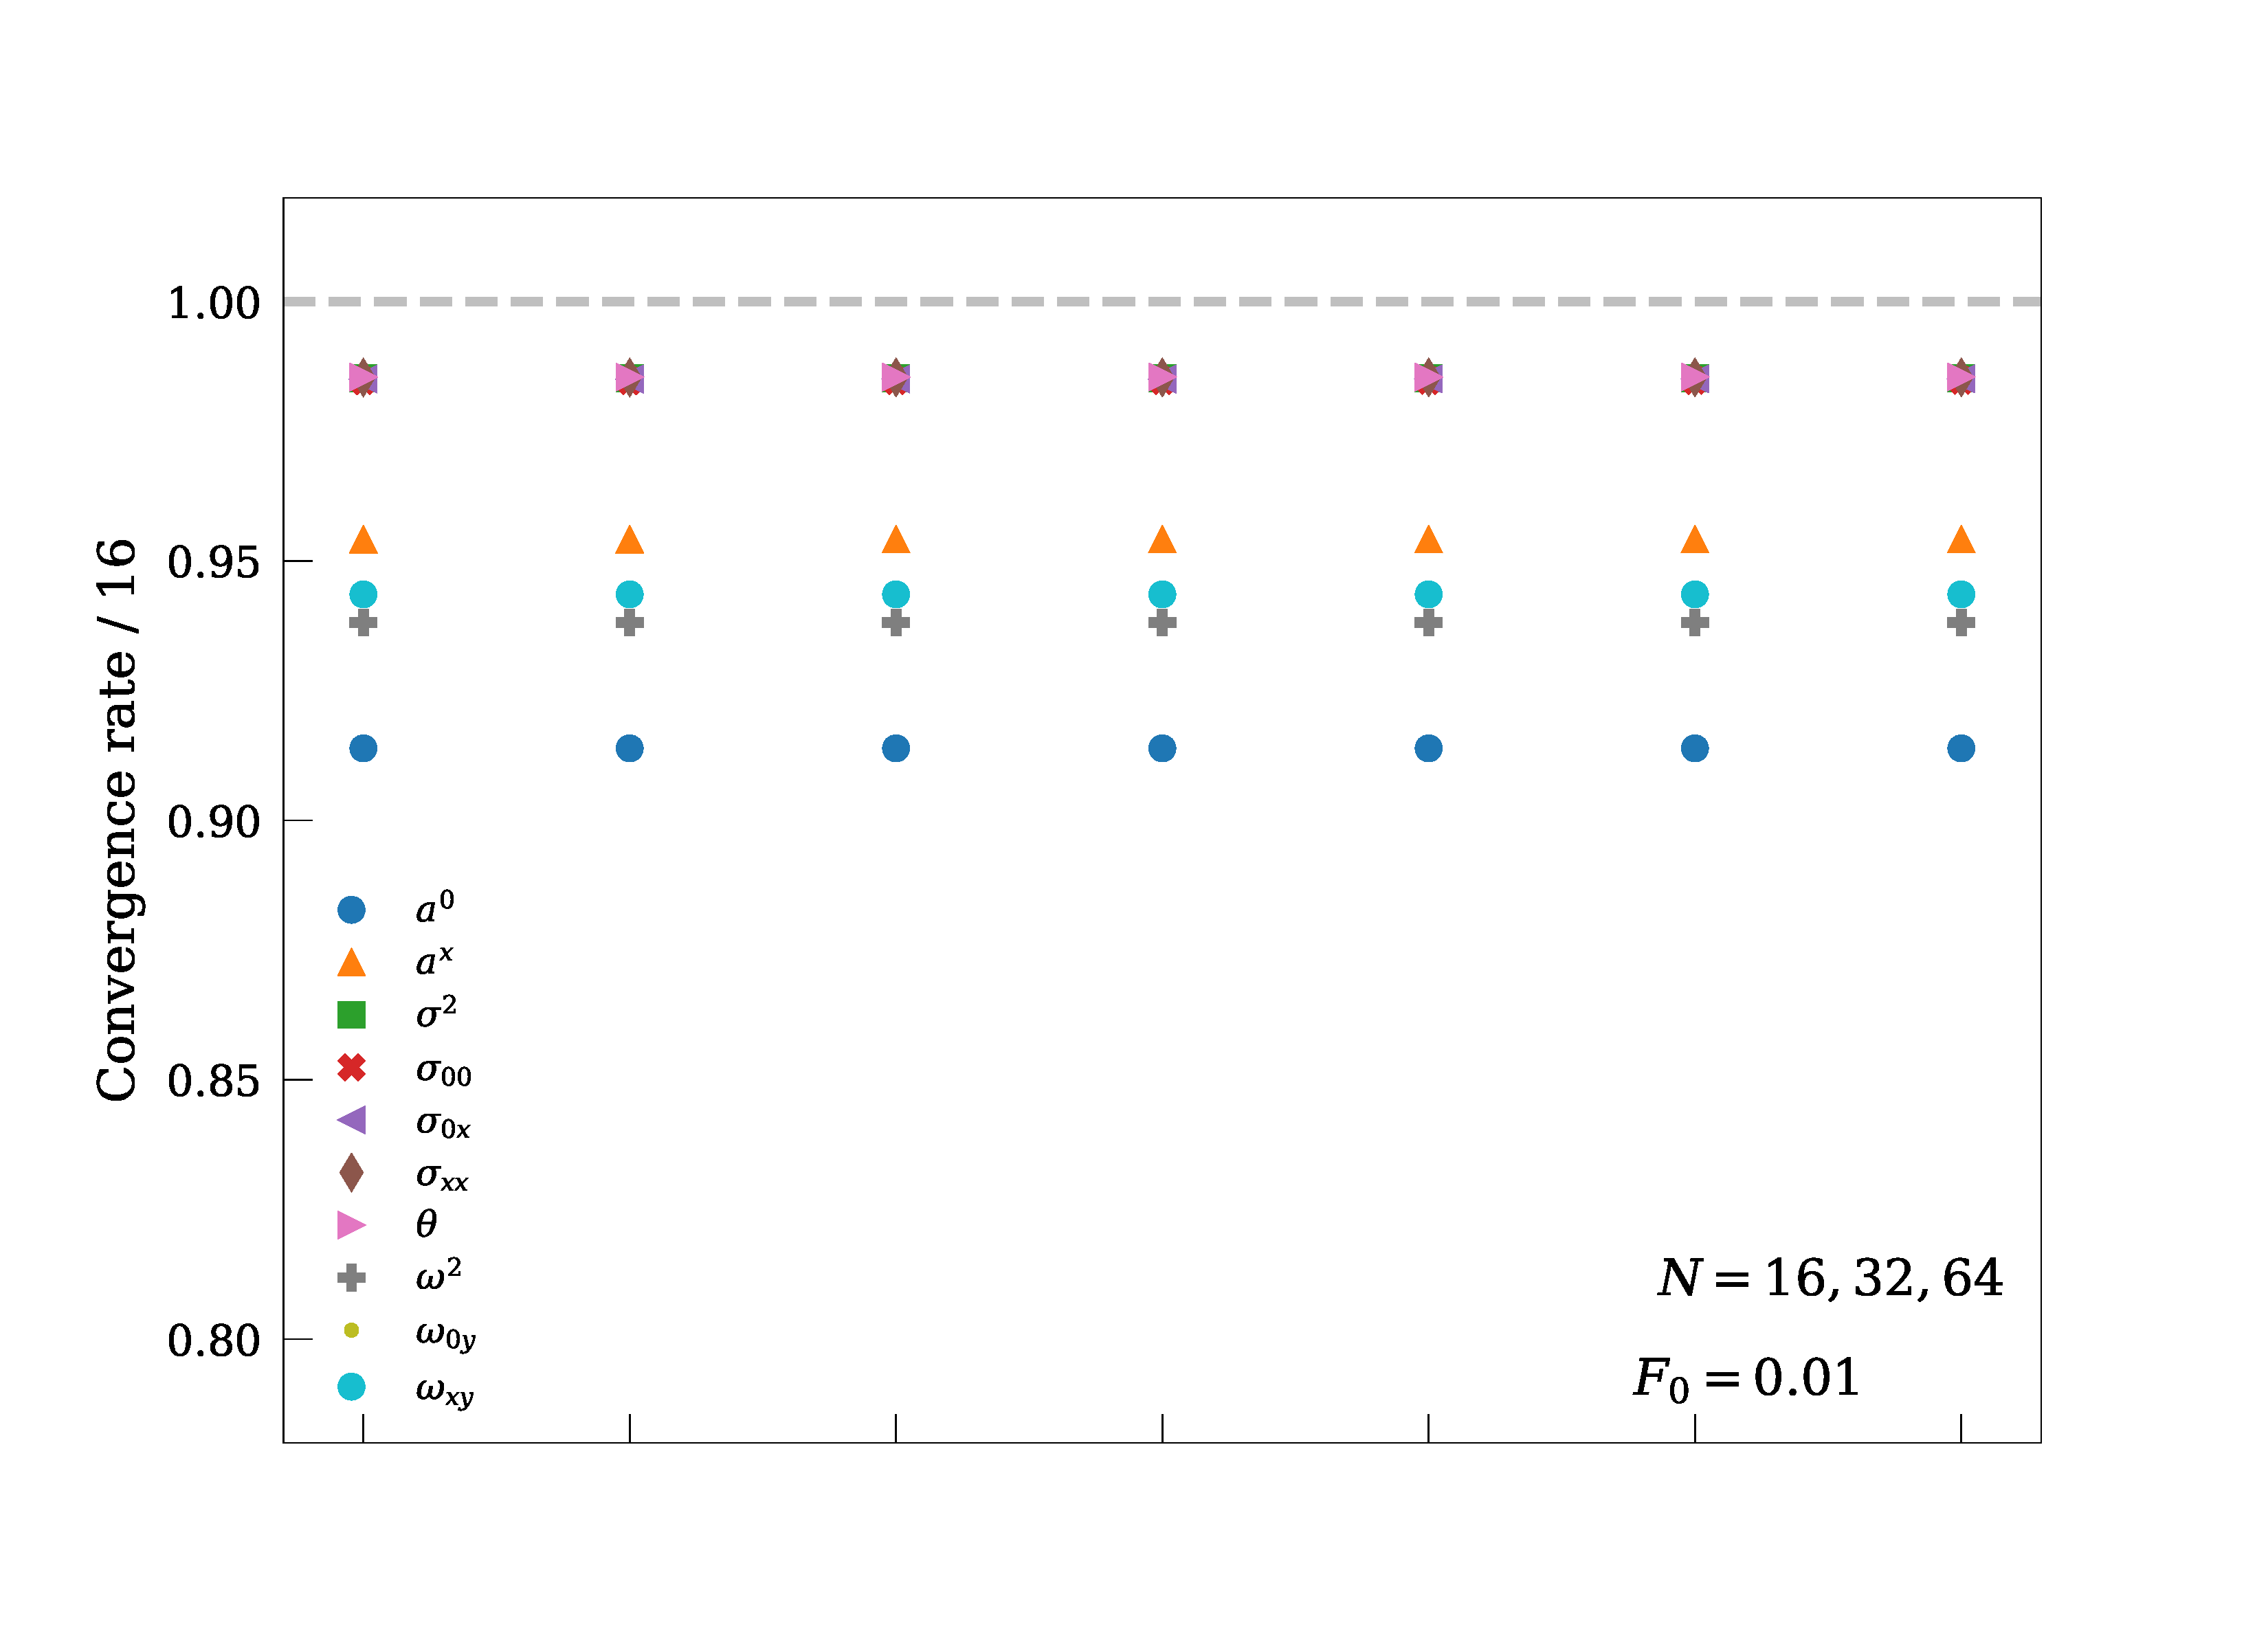
\includegraphics[width=\linewidth]{figures/HayTest_convergence_N16_32_64_amp1em2_allvars_noR.pdf}
    \end{subfigure}%
    \begin{subfigure}{.5\textwidth}
          \centering
          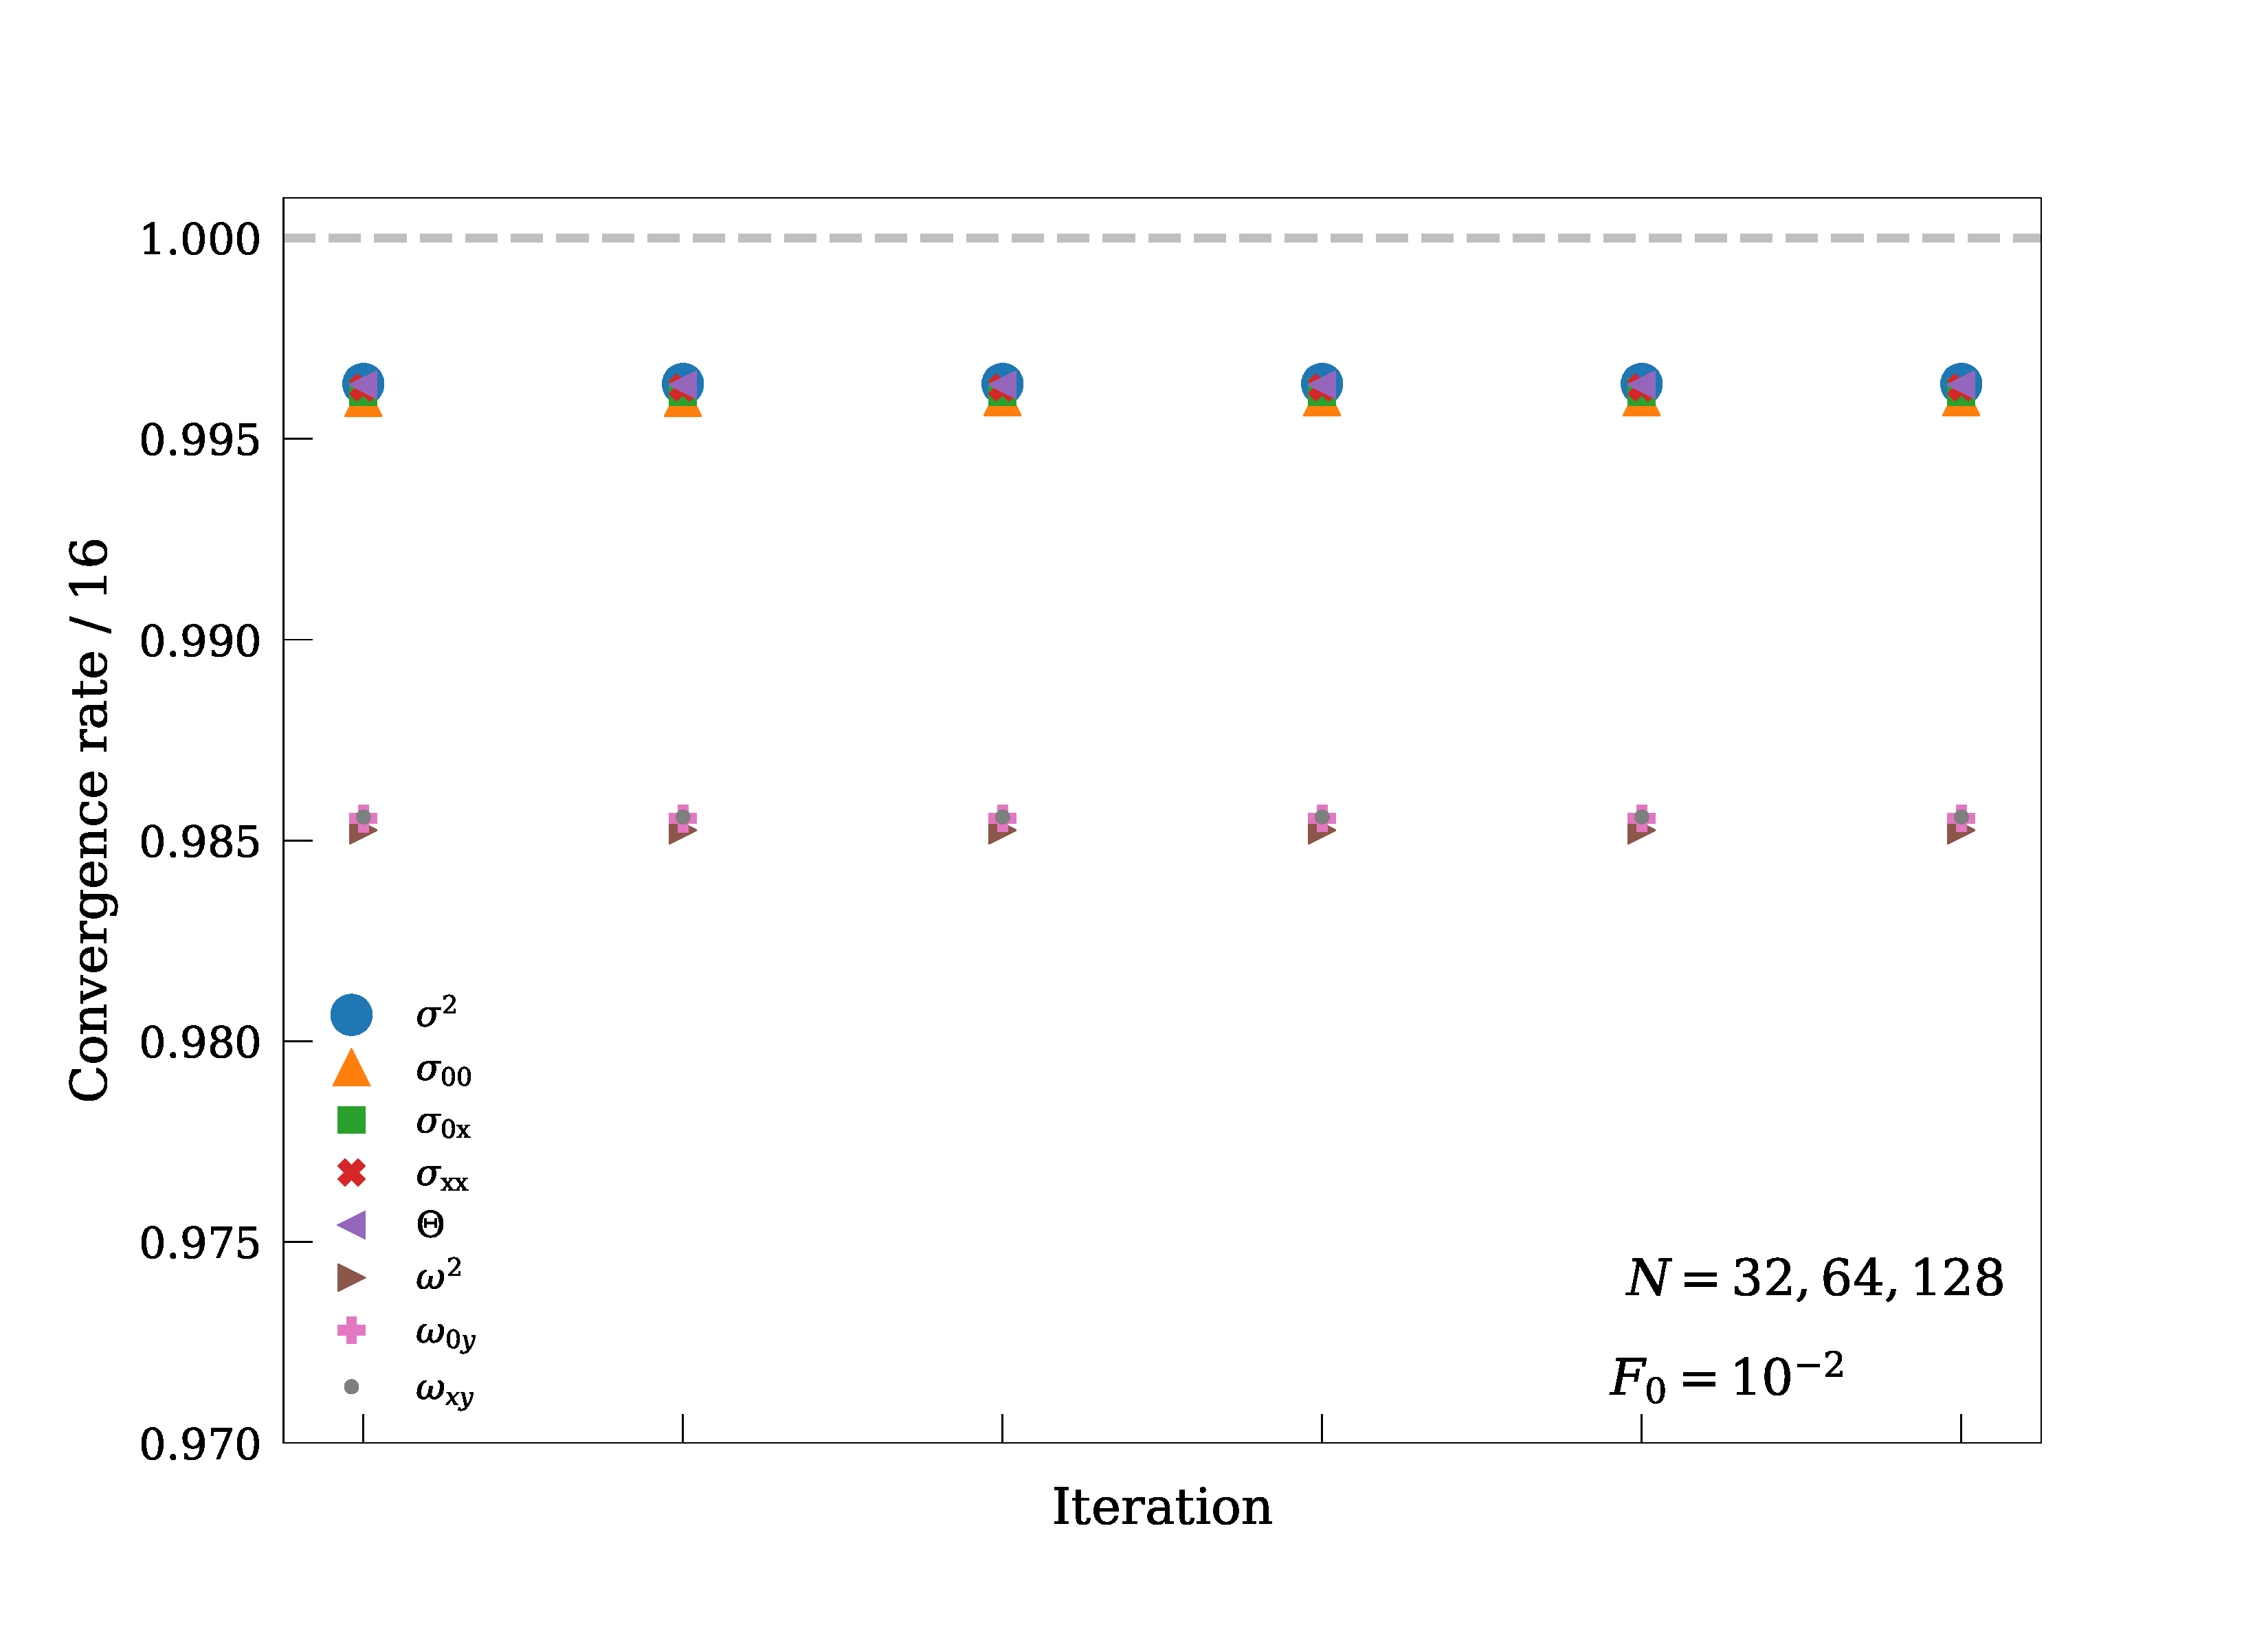
\includegraphics[width=\linewidth]{figures/HayTest_convergence_N32_64_128_amp1em2_allvars_noR.pdf}
    \end{subfigure}
    \caption{Convergence rate, $C$, relative to the expected value for fourth-order convergence for all variables studied here in the arbitrary metric test. We show resolutions $N=16,32,64$ (left panel) and $N=32, 64, 128$ (right panel), both for an amplitude of $F_0=10^{-2}$. We see an improvement in the convergence with increasing resolution, and the convergence is independent of $F_0$, as long as $F_0<0.1$ (see main text).}
    \label{fig:HayTest_Convergence_smallamp}
\end{figure}

The left panel of Figure~\ref{fig:HayTest_Convergence_smallamp} shows the convergence rate for the kinematical variables calculated using resolutions $N=16,32,64$ and the right panel shows $N=32,64,128$. We see an improvement in the convergence rate with an increase in resolution (left to right). The results here are for an amplitude $F_0=10^{-2}$, however we see identical convergence behaviour for all amplitudes $F_0\leq10^{-2}$. We note we show the convergence for the acceleration $a^\mu$ in the left panel, but not the right. Due to additional memory storage (and Hayley being lazy to write a quick way around this), running $N=128$ for the test case was significantly slower. We expect similar behaviour to the other variables in that convergence improves with an increase in resolutions used. 

%%%%%%% multi-panel figure
\begin{figure}[h!]
    \begin{subfigure}{.5\textwidth}
          \centering
          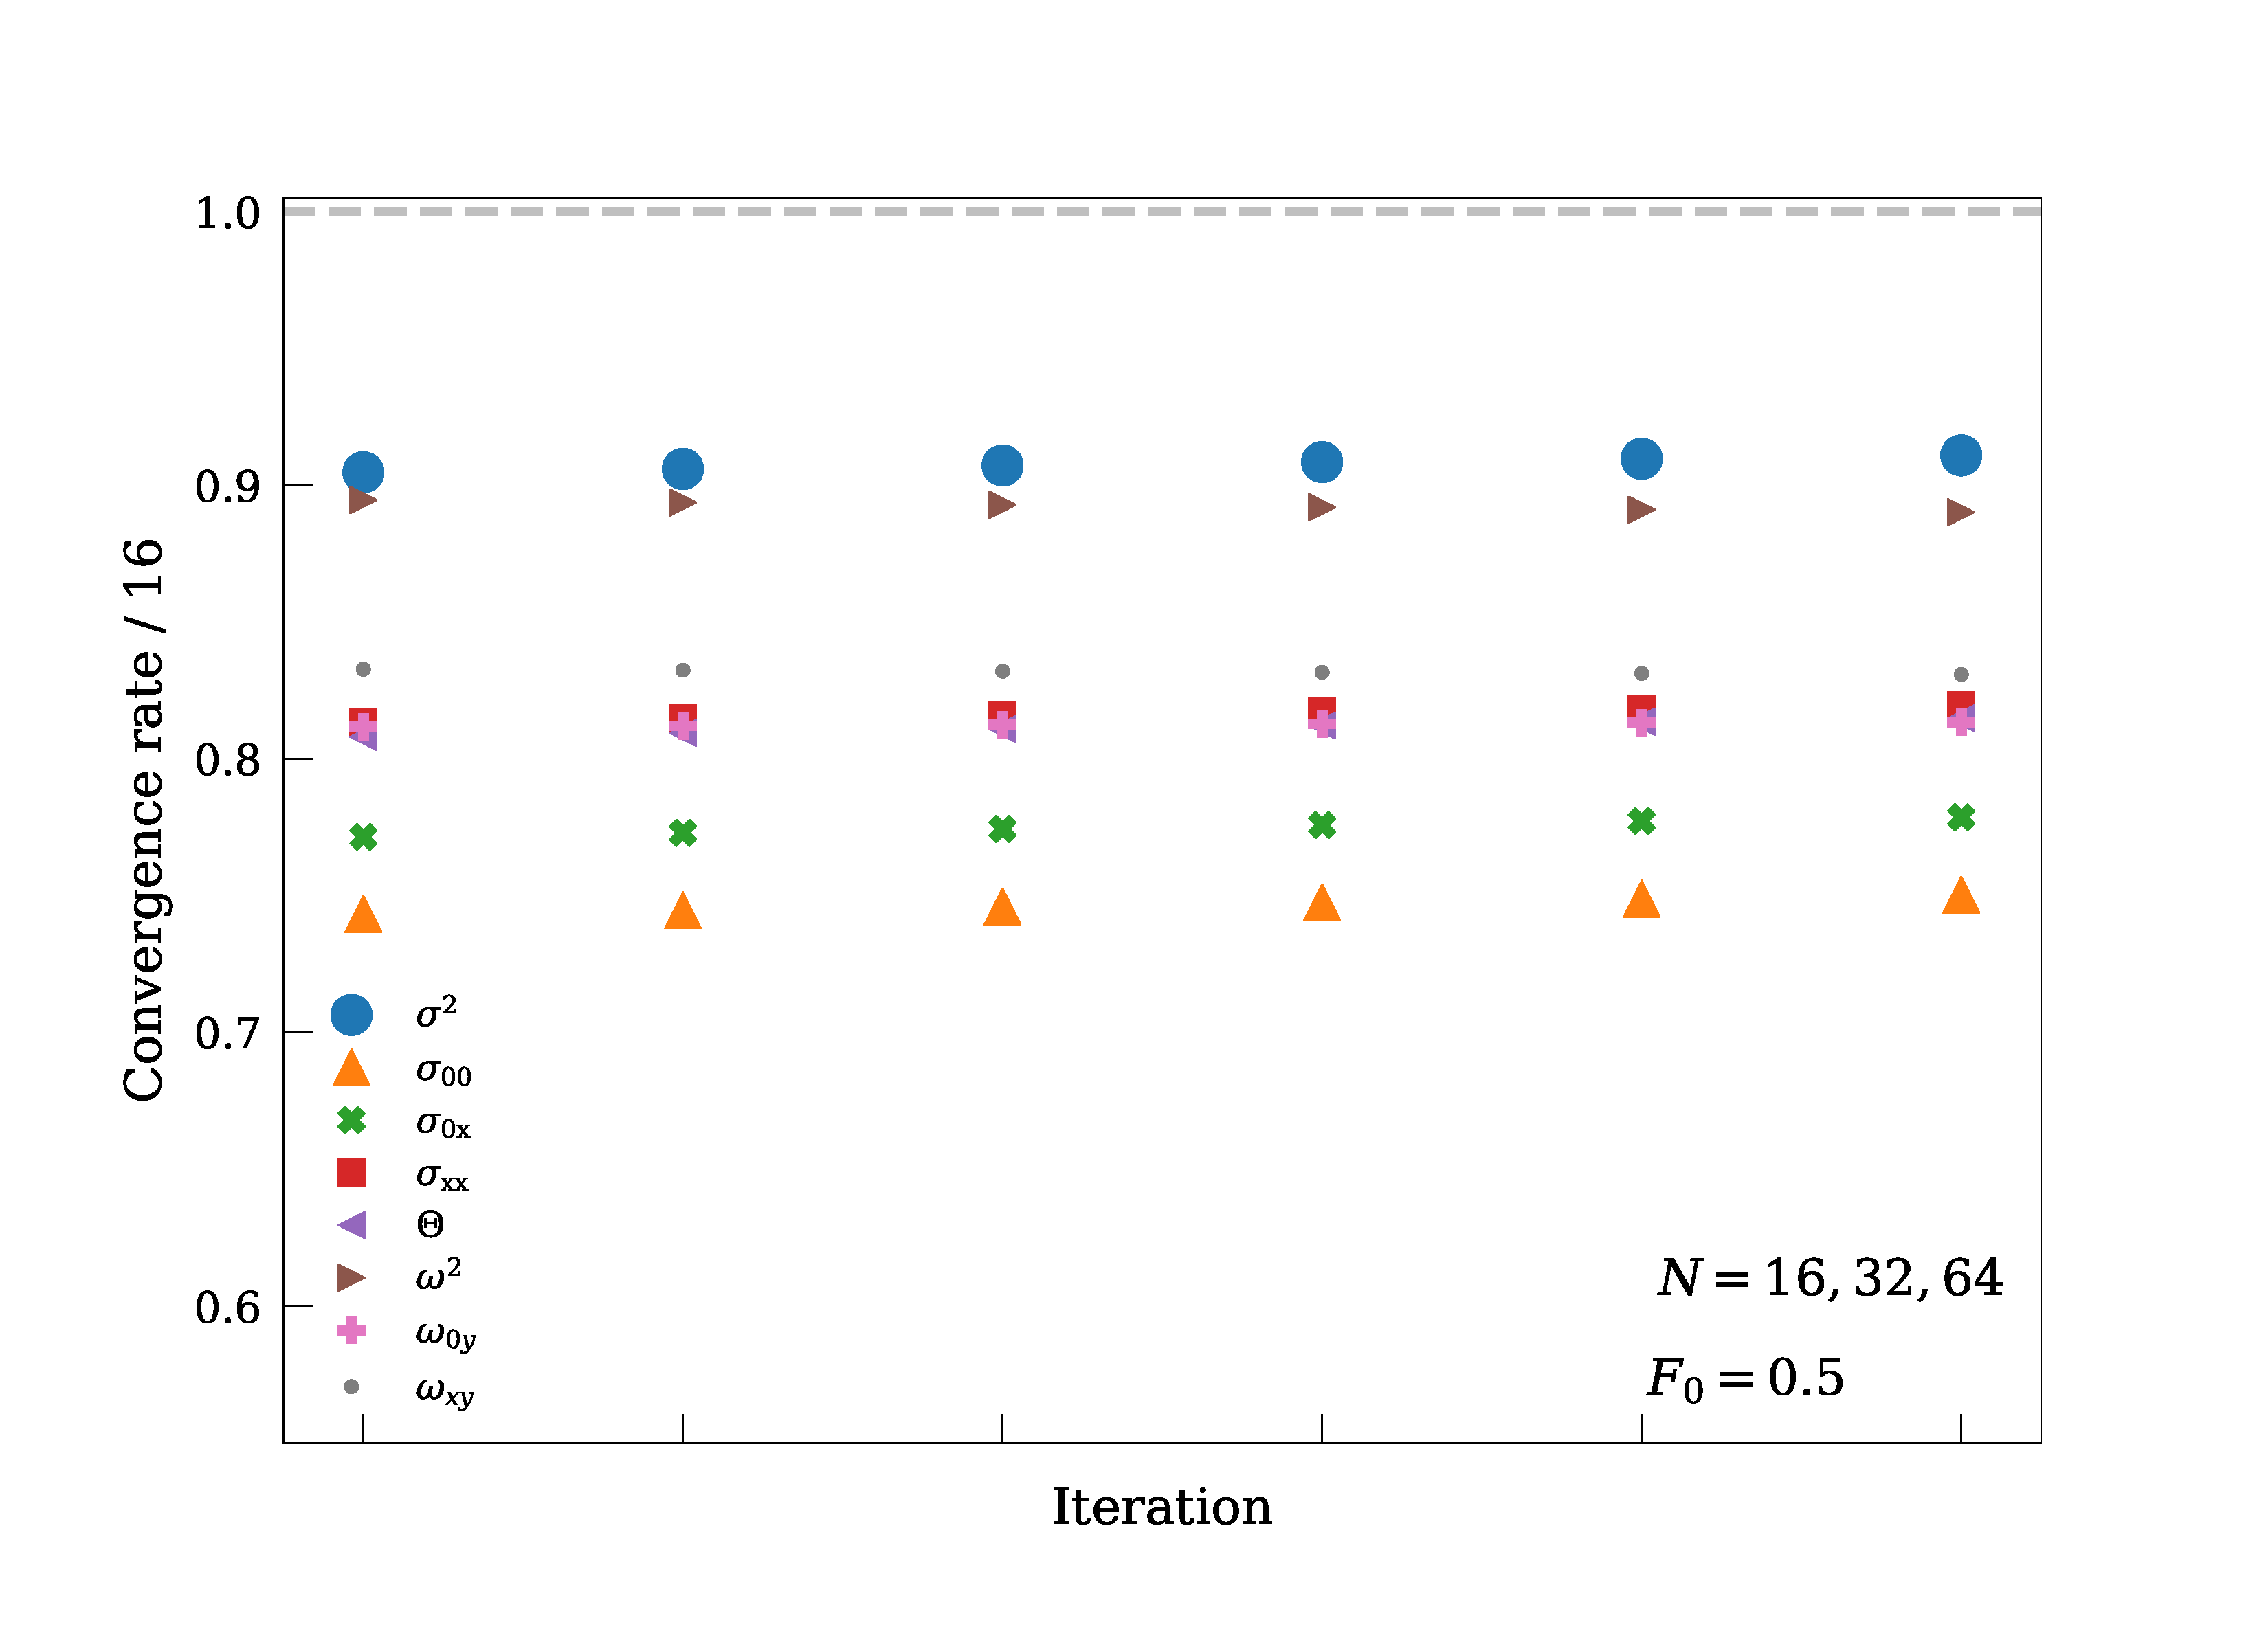
\includegraphics[width=\linewidth]{figures/HayTest_convergence_N16_32_64_amp0p5_allvars_noR.pdf}
    \end{subfigure}%
    \begin{subfigure}{.5\textwidth}
          \centering
          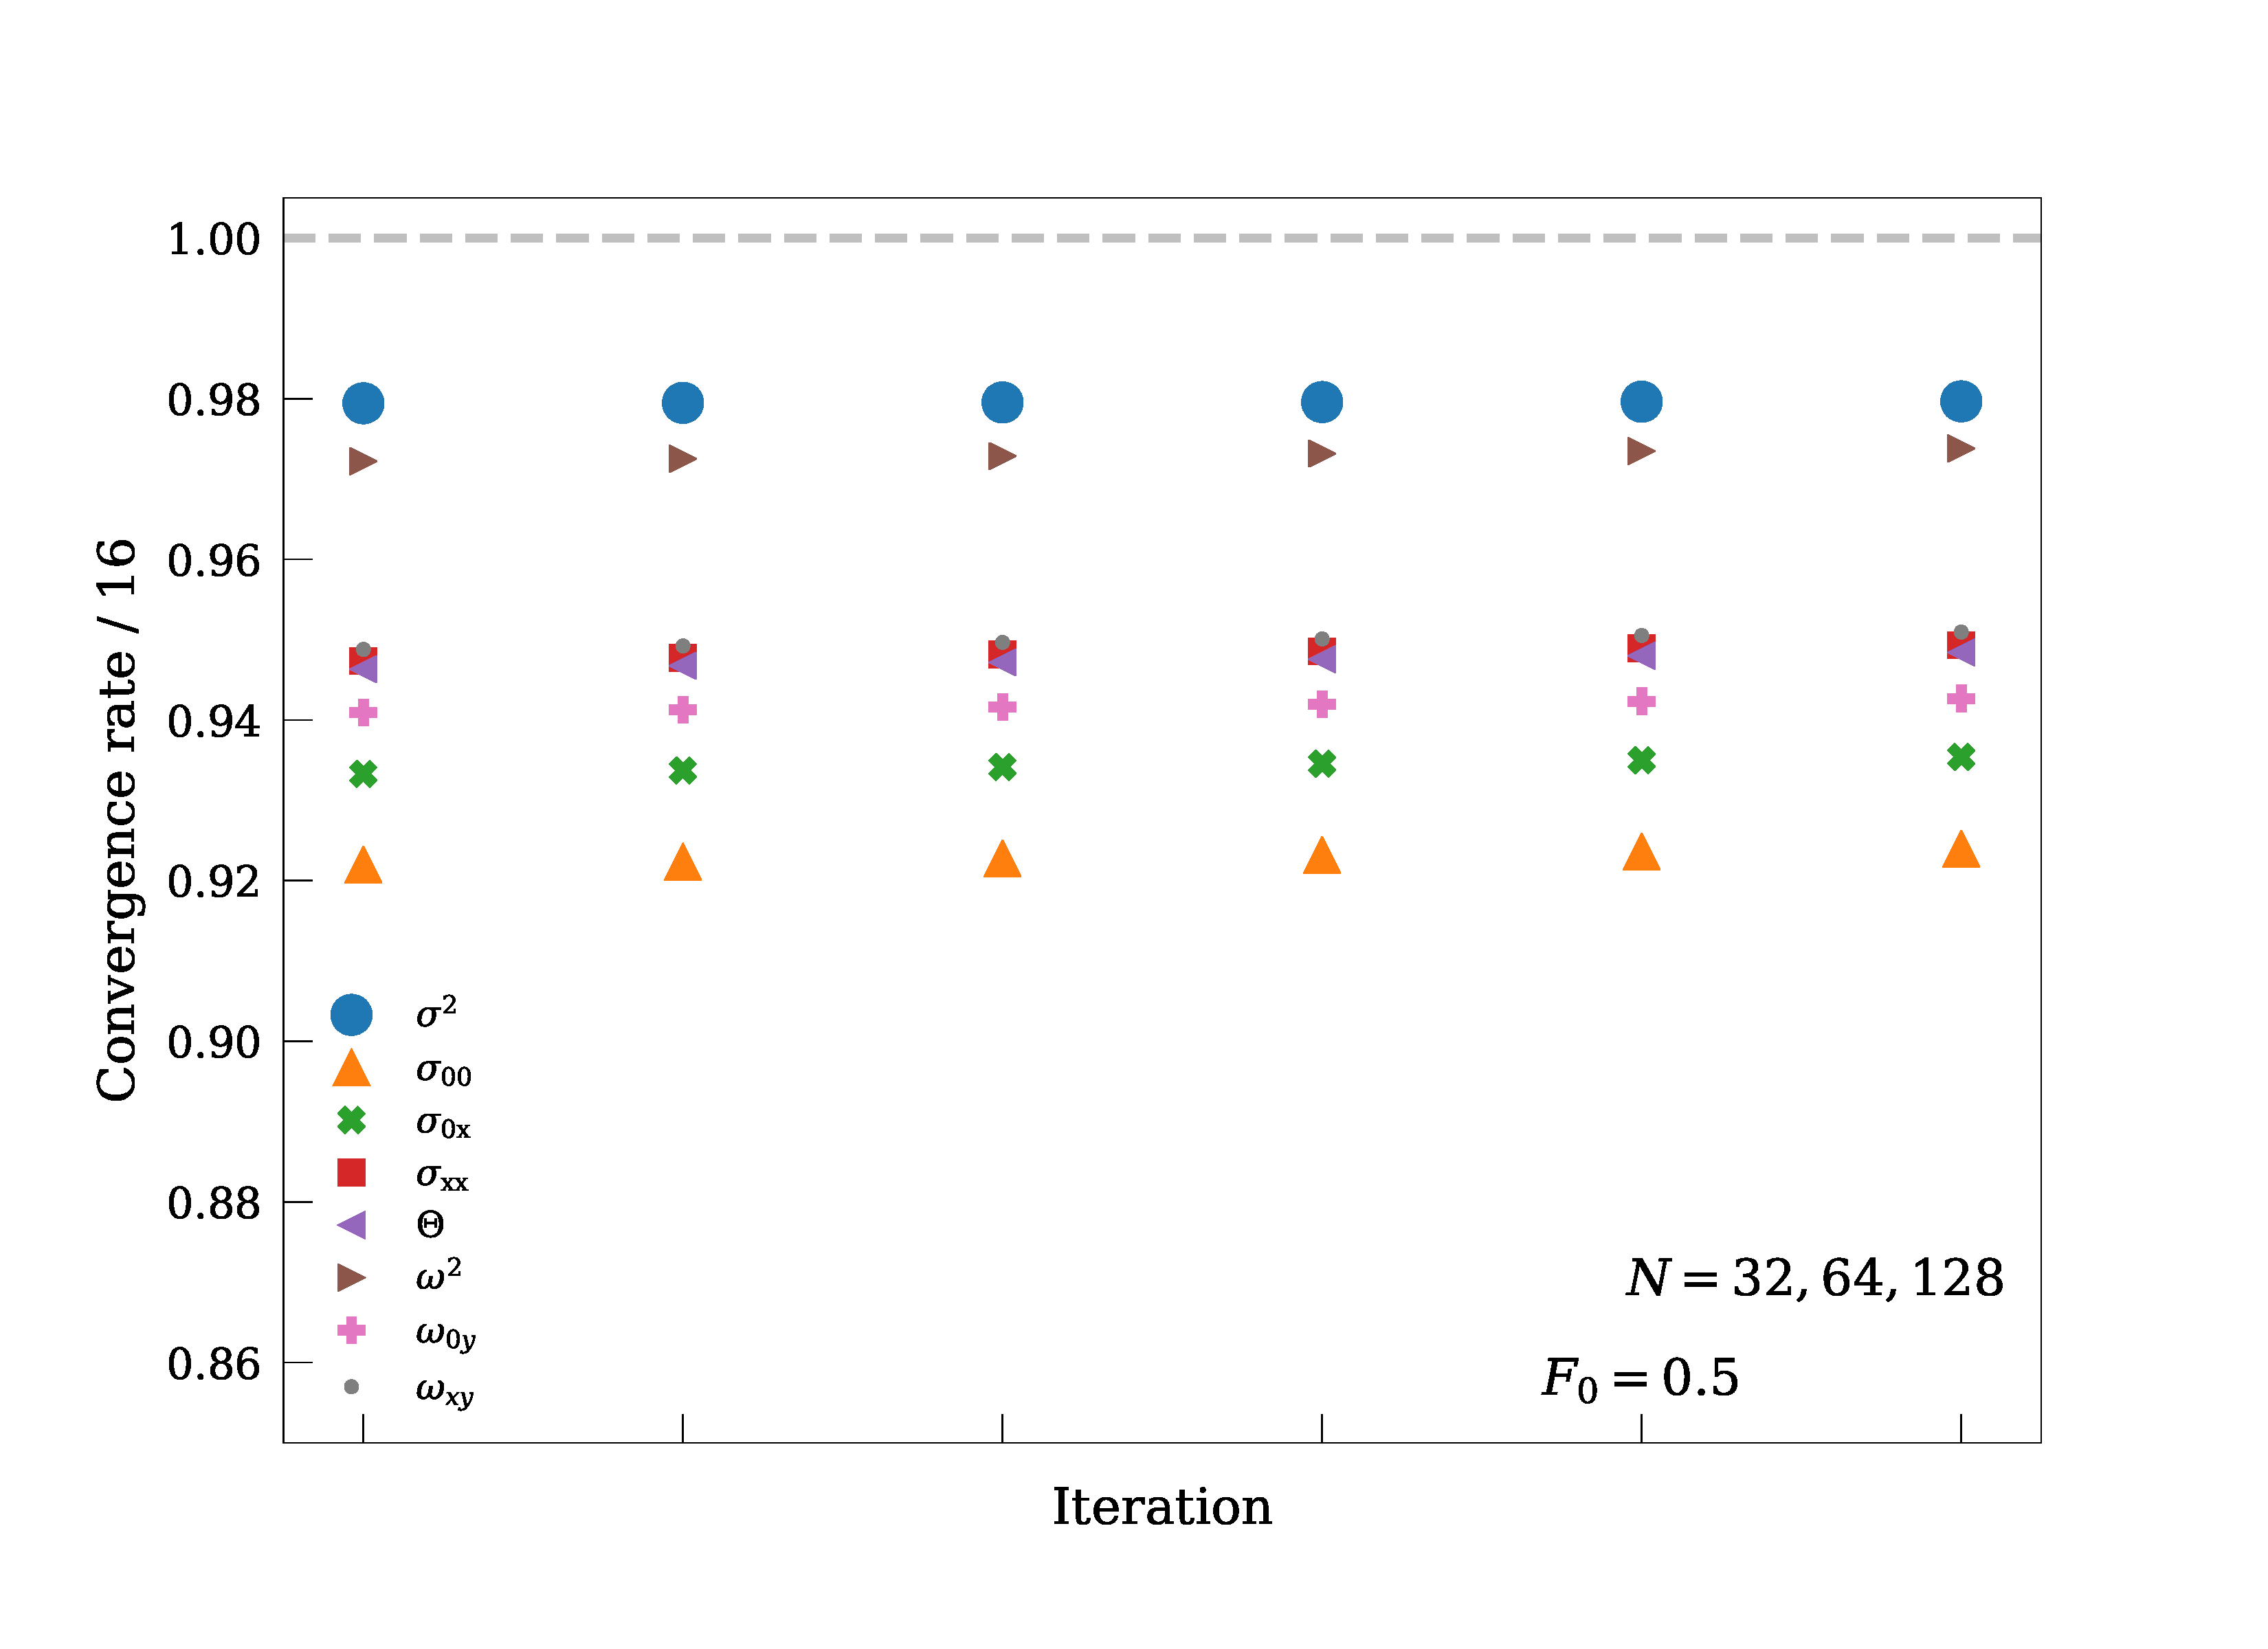
\includegraphics[width=\linewidth]{figures/HayTest_convergence_N32_64_128_amp0p5_allvars_noR.pdf}
    \end{subfigure}
    \caption{Convergence rate, $C$, relative to the expected value for fourth-order convergence for all variables studied here in the arbitrary metric test. We show resolutions $N=16,32,64$ (left panel) and $N=32, 64, 128$ (right panel), both for an amplitude of $F_0=0.5$.}
    \label{fig:HayTest_Convergence_amp0p5}
\end{figure}

Figure~\ref{fig:HayTest_Convergence_amp0p5} shows the convergence rate when we increase the amplitude to $F_0=0.5$. The left panel shows the convergence calculated using resolutions $N=16,32,64$ and the right panel shows $N=32,64,128$. In this case, the velocity becomes relativistic (since $v^x=F$) and consequently the \emph{gradients} of the variables studied here are extremely steep. We therefore need a higher resolution to sample these gradients, which is illustrated in the improvement of the convergence rate between the left and right panels of Figure~\ref{fig:HayTest_Convergence_amp0p5}. We would need an even higher resolution to achieve the same convergence as is seen for the smaller amplitudes in Figure~\ref{fig:HayTest_Convergence_smallamp}. 

\begin{figure}[h!]
	\centering
  	 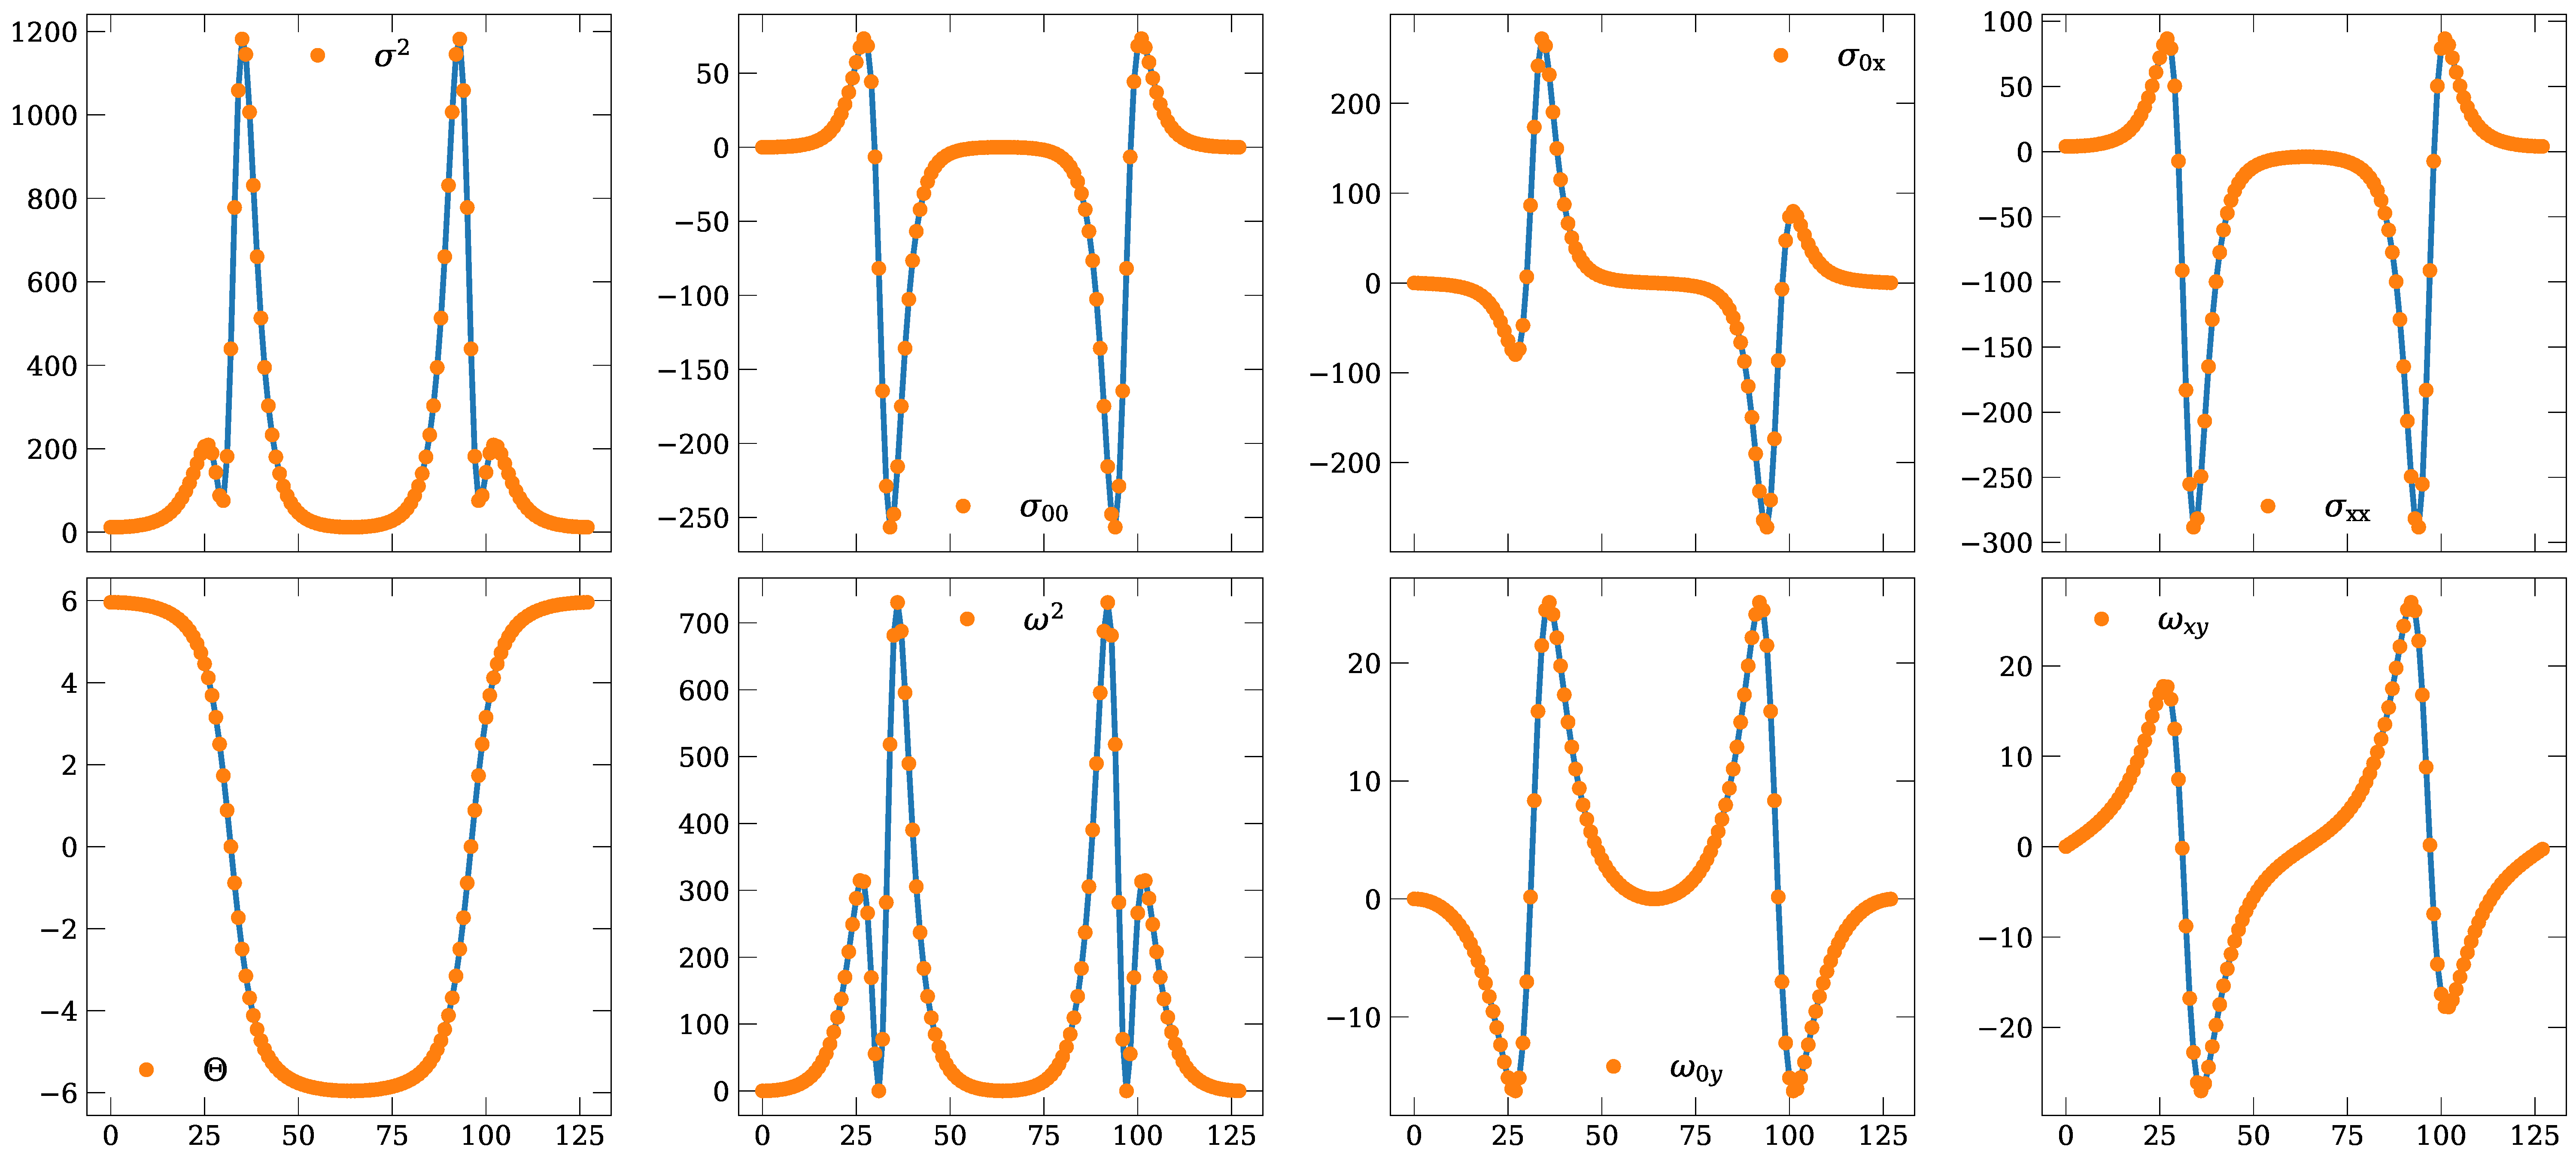
\includegraphics[width=\textwidth]{figures/HayTest_8panel_xslices_allvars_N128_amp1_t0p003125.pdf} 
  	 \caption{The most extreme case studied here for the arbitrary metric test, with amplitude $F_0=0.95$ for resolution $N=128$. Each panel shows an x-slice halfway through the domain in y and z for each kinematical variable studied in this test. Orange dots are the \mesc\, solutions and solid blue curves are the corresponding analytic solution.}
 	  \label{fig:Haytest_8panel}
\end{figure}

To demonstrate this, in Figure~\ref{fig:Haytest_8panel} we show the most extreme case we studied with amplitude $F_0=0.95$ for resolution $N=128$, which exhibits similar (yet amplified) behaviour to $F_0=0.5$. Each panel shows a one-dimensional $x$-slice for each kinematical variable, as indicated in each legend. The orange dots are the solution from \mesc, and the solid curve is the corresponding analytic solution. In this case we see convergence $C \sim 9$ (where we expect 16) for resolutions $N=32,64,128$. We notice that the areas where the gradients are very steep are sampled by only a few points, and so we need an even higher resolution to capture these extreme configurations.

%%%%%%% multi-panel figure
\begin{figure}[h!]
    \begin{subfigure}{.5\textwidth}
          \centering
          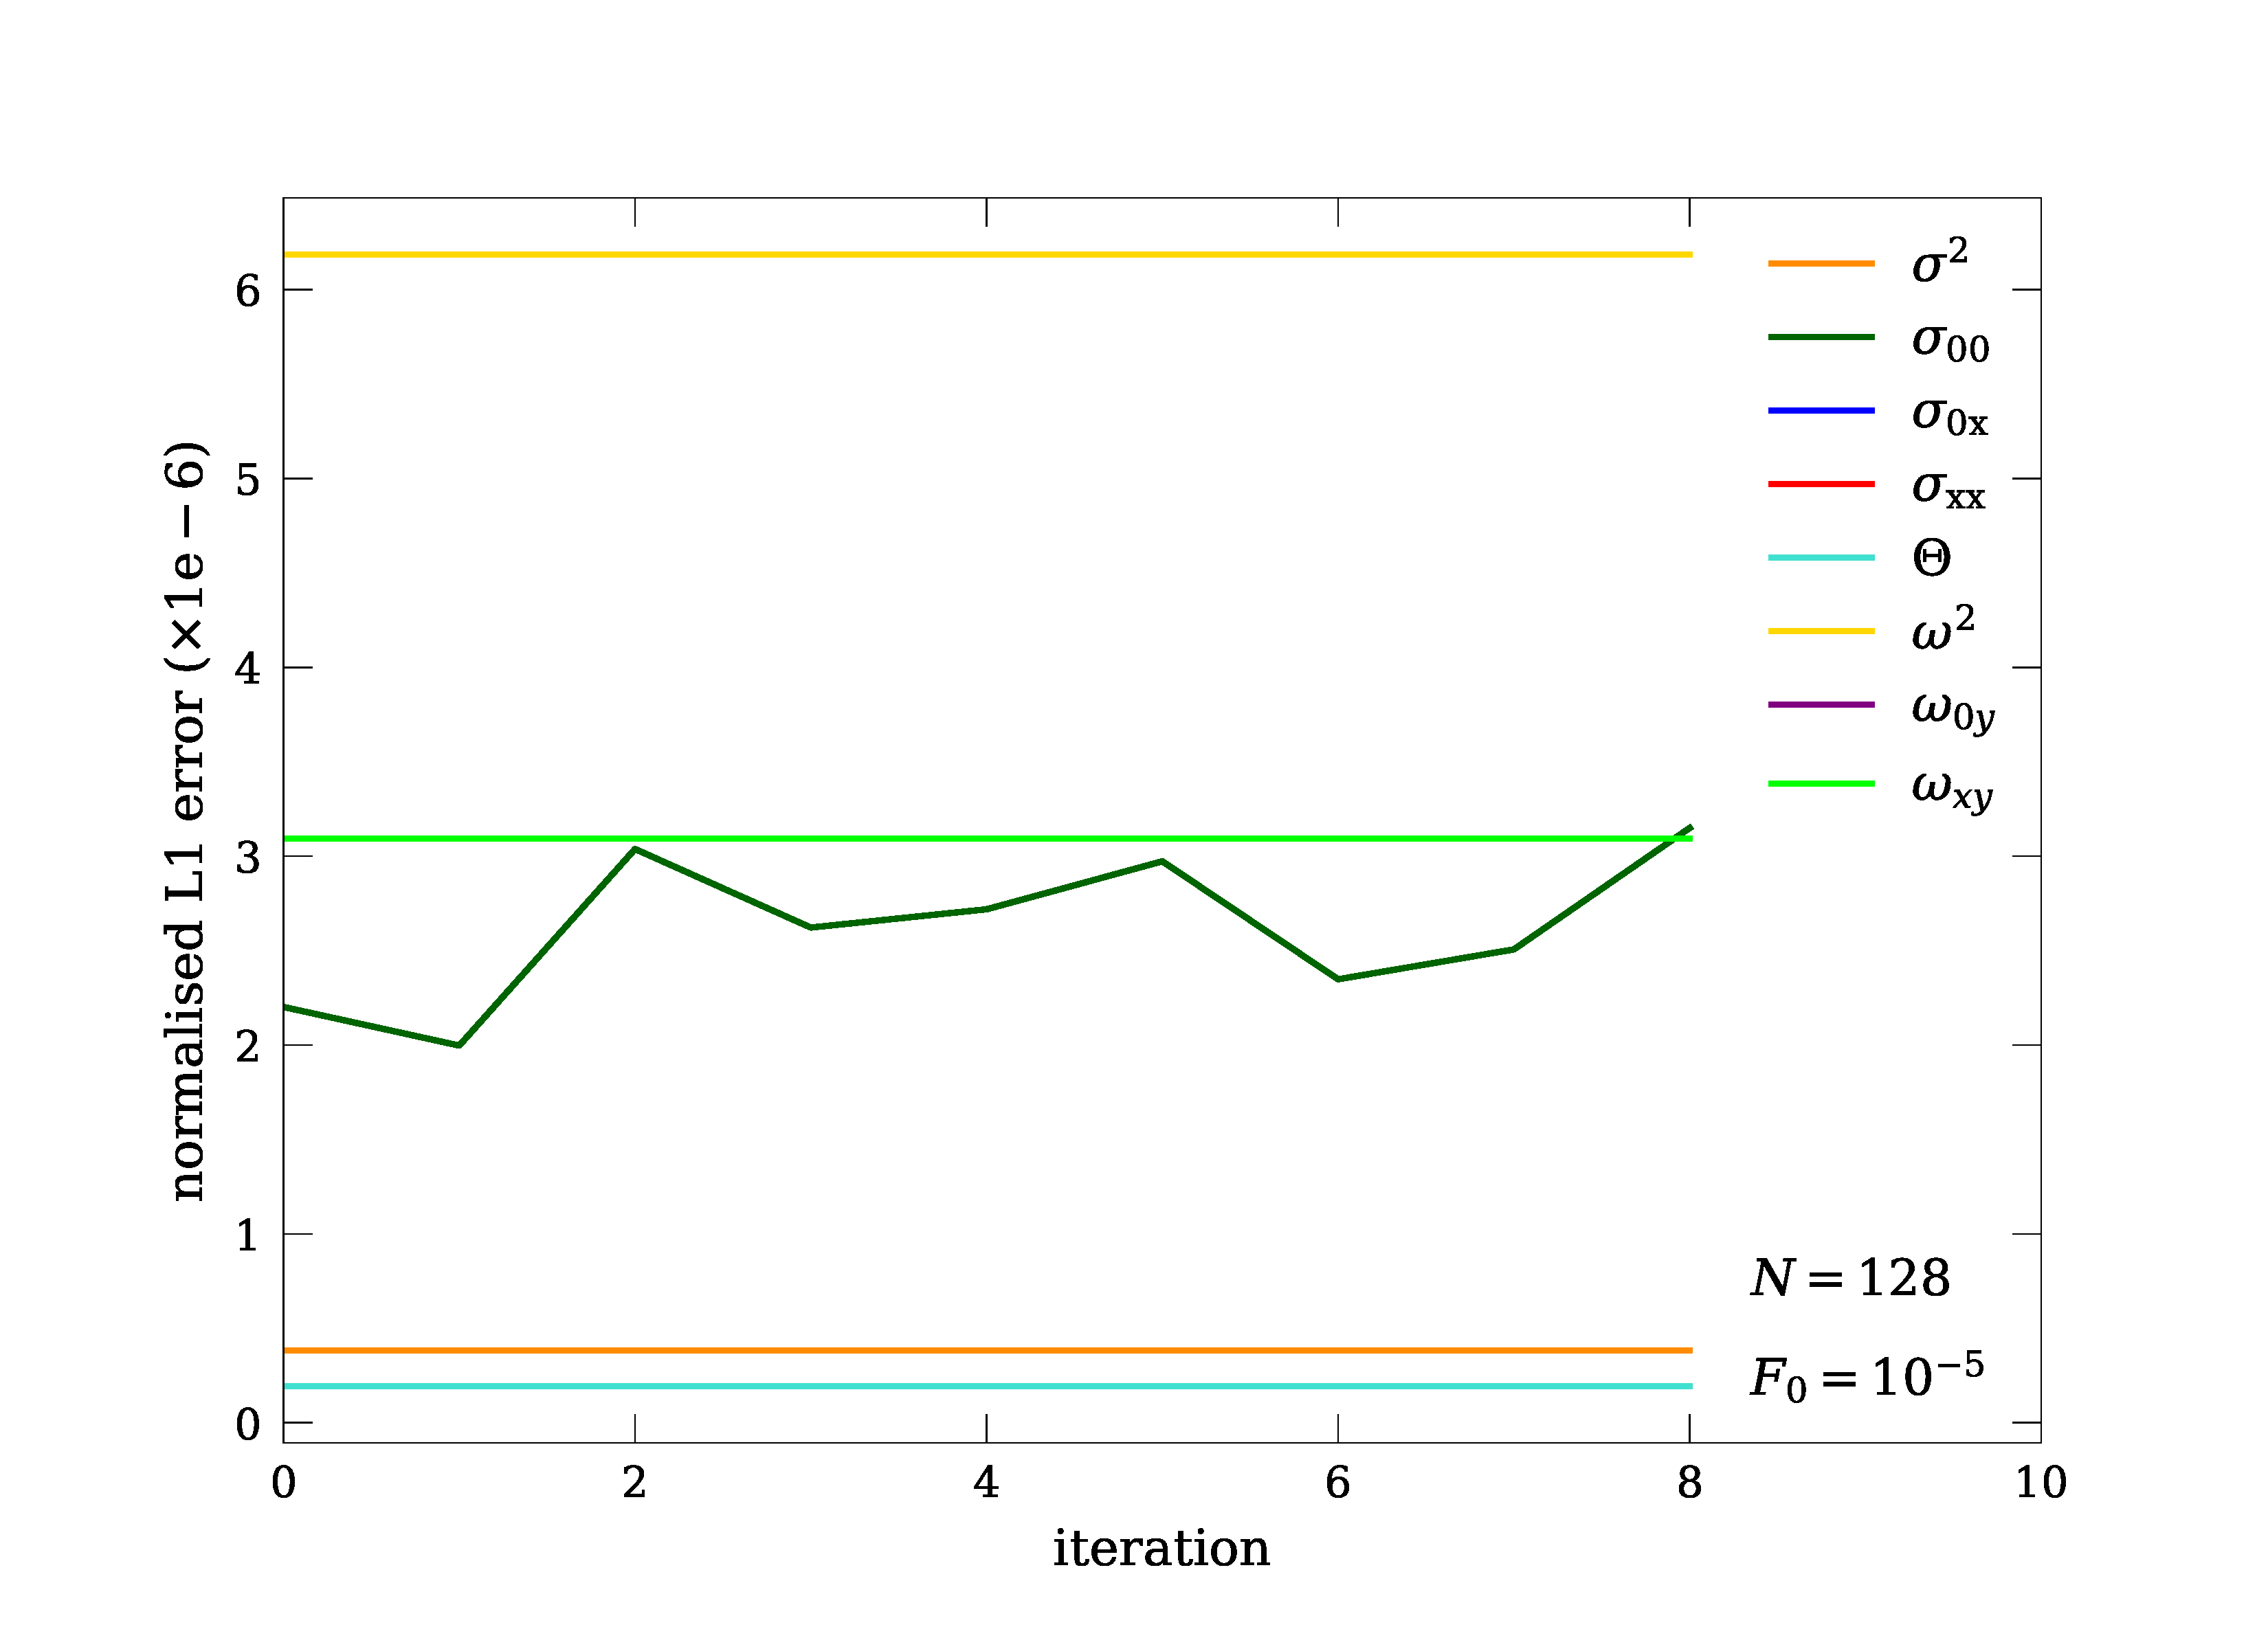
\includegraphics[width=\linewidth]{figures/HayTest_normedL1error_N128_amp1em5_allvars_noR.pdf}
    \end{subfigure}%
    \begin{subfigure}{.5\textwidth}
          \centering
          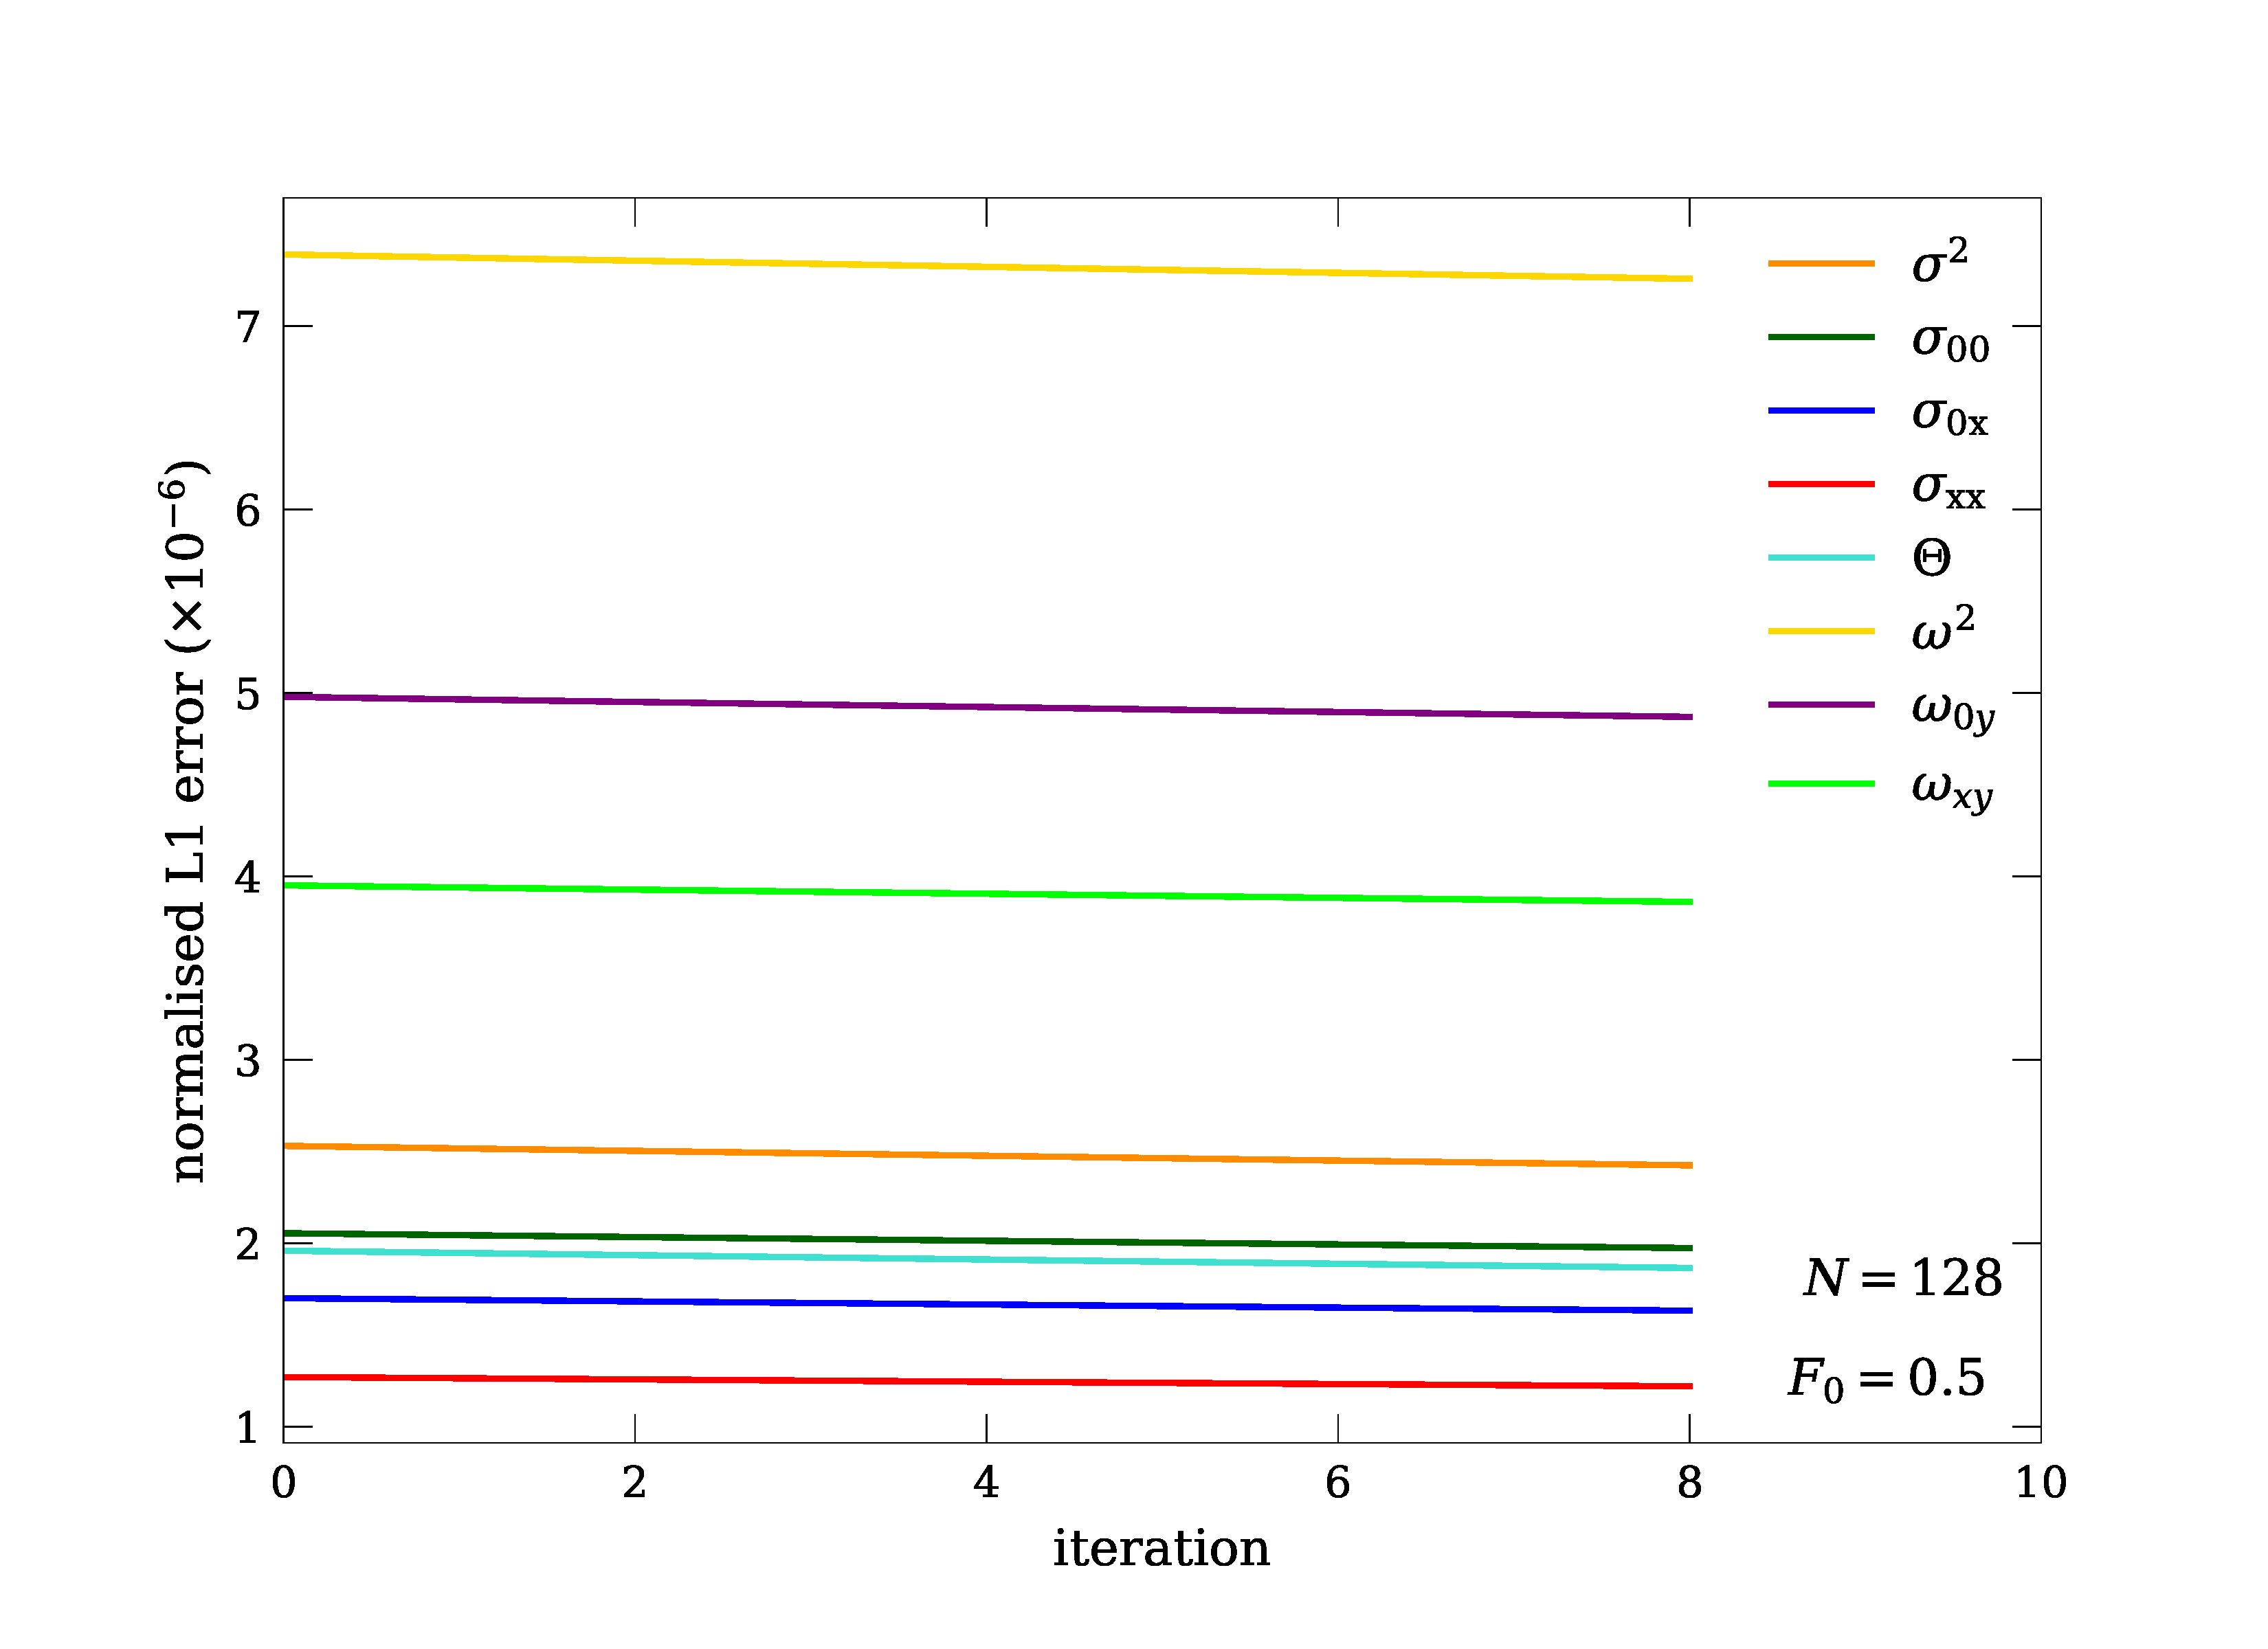
\includegraphics[width=\linewidth]{figures/HayTest_normedL1error_N128_amp0p5_allvars_noR.pdf}
    \end{subfigure}
    \caption{Normalised L1 error for all variables studied here for the arbitrary metric test as a function of iteration. Both panels are for resolution $N=128$, the highest resolution used here. The left panel is for an amplitude $F_0=10^{-5}$, and the right panel for $F_0=0.5$. We notice that the error increases only slightly for a significant increase in the amplitude.}
    \label{fig:HayTest_L1error}
\end{figure}

Figure~\ref{fig:HayTest_L1error} shows the normalised L1 error for all kinematical variables as a function of time. Both panels are for the highest resolution we use here of $N=128$, and the left panel shows an amplitude $F_0=10^{-5}$, and the right panel $F_0=0.5$. While the convergence is affected significantly in this case, the L1 error is controlled when increasing the amplitude by 4 orders of magnitude, and increases only slightly. We note we have excluded the L1 error for the acceleration $a^\mu$ in this plot, for reasons stated above. However, the L1 error for $a^0$ and $a^x$ are smaller than all other kinematical variables in Figure~\ref{fig:HayTest_L1error} for $N=64$ and $F_0=0.01$.





\addcontentsline{toc}{section}{References}
\bibliographystyle{apalike}
%\bibliographystyle{klunamed}
\bibliography{litreview.bib}

\end{document}
